\documentclass[a4paper]{article}

\usepackage[T1]{fontenc}
\usepackage[utf8]{inputenc}
\usepackage{emmt-unicode}

\usepackage[authoryear,round]{natbib}

\usepackage{amsmath,amsfonts} % before newtx, newtexmath, newtxtext
\usepackage{mathtools}

%\usepackage[garamondx]{newtx}
%\usepackage[ebgaramond]{newtx}
%\usepackage{lmodern}
\usepackage{libertine}

\usepackage{stmaryrd}
\usepackage{bm} % load after all math to give access to bold math

\usepackage[hyperref]{xcolor}
\colorlet{textfg}{black}
\colorlet{textbg}{white}
\definecolor{OwlRed}{RGB}{255,92,168}
\definecolor{OwlGreen}{RGB}{90,168,0}
\definecolor{OwlBlue}{RGB}{0,152,233}
\definecolor{OwlYellow}{RGB}{242, 147,24}
\colorlet{OwlViolet}{OwlRed!50!OwlBlue}
\colorlet{OwlBrown}{OwlRed!50!OwlGreen}
\colorlet{OwlOrange}{OwlRed!50!OwlYellow}
\colorlet{OwlCyan}{OwlGreen!50!OwlBlue}

\usepackage[unicode,colorlinks=true,allcolors=OwlBlue]{hyperref}

\usepackage{tikz}
\usetikzlibrary{math} % needed for tikz variables and math expressions
\tikzset{%
  view3d/.style={x={(1cm,0cm)},y={(0cm,1cm)},z={(0.8cm,-0.3cm)}},
  grid lines/.style={very thin, color=textfg!50!textbg}
}

\usepackage[breakable,theorems,skins]{tcolorbox}
%\tcbuselibrary{breakable} % for breakable boxes
%\tcbuselibrary{theorems}  % for \tcboxmath{
%\tcbuselibrary{skins}     % for `enhanced jigsaw` engine

\newtcolorbox{examplebox}[1]{
  enhanced jigsaw, sharpish corners, breakable,
  %colframe=black!65!white, colback=black!5!white,
  % bottomrule at break=0mm, toprule at break=0pt,
  fonttitle=\bfseries, title={#1}}

\newcommand{\oops}[1]{{\color{purple}#1}}

\usepackage{xspace}
\newcommand*{\latinabbreviation}[1]{\emph{#1}\xspace}
\newcommand*{\ie}{\latinabbreviation{i.e.}}
\newcommand*{\eg}{\latinabbreviation{e.g.}}
\newcommand*{\cf}{\latinabbreviation{cf.}}

%\newcommand{\V}[1]{\vec{#1}}
\newcommand*{\V}[1]{\boldsymbol{#1}}
\newcommand*{\M}[1]{\mathbf{#1}}
%\newcommand*{\TransposeLetter}{\mathrm{T}}
\newcommand*{\TransposeLetter}{\top}
\newcommand*{\T}{^\TransposeLetter}

%% Parentheses:
%\def\Paren{}\let\Paren\undefined
\DeclarePairedDelimiterX{\Paren}[1]{(}{)}{#1}
\DeclarePairedDelimiterX{\Brace}[1]{\{}{\}}{#1}
\DeclarePairedDelimiterX{\Brack}[1]{[}{]}{#1}
%\DeclarePairedDelimiterX{\Abs}[1]{\rvert}{\lvert}{#1}
\DeclarePairedDelimiterX{\Abs}[1]{|}{|}{#1}
\DeclarePairedDelimiterX{\Norm}[1]{\lVert}{\rVert}{#1}
\DeclarePairedDelimiterX{\Avg}[1]{\langle}{\rangle}{#1}
\DeclarePairedDelimiterX{\Round}[1]{\lfloor}{\rceil}{#1}
\DeclarePairedDelimiterX{\Floor}[1]{\lfloor}{\rfloor}{#1}
\DeclarePairedDelimiterX{\Ceil}[1]{\lceil}{\rceil}{#1}
\DeclarePairedDelimiterX{\Inner}[2]{\langle}{\rangle}{#1,#2}
\DeclarePairedDelimiterX{\IntRange}[1]{\llbracket}{\rrbracket}{#1}
\DeclarePairedDelimiterX{\Group}[1]{\lgroup}{\rgroup}{#1}
%\DeclarePairedDelimiterX{\FrobNorm}[1]{\lVert}{\rVert_{\Tag{F}}}{#1}
%% A list \List{ELEM}{START}{END}
\DeclarePairedDelimiterXPP{\List}[3]{}{\{}{\}}{_{#2,…,#3}}{#1}

\newcommand*{\delimsize}{}
\newcommand*{\suchthat}{\,\vert\,} % compact version
\newcommand*{\SuchThat}{\,\delimsize\vert\,} % autoscale to surrounding version
\newcommand*{\given}{\,\vert\,} % compact version
\newcommand*{\Given}{\,\delimsize\vert\,} % autoscale to surrounding version
%\newcommand*{\given}{\mathbin{\vert}}
%\newcommand*{\Given}{\mathrel{\delimsize\vert}} % autoscale to surrounding version

% For function definitions: $f \from E \to F$.
\newcommand*{\from}{{:}\:}

%% Upright letters.
\newcommand*{\mathd}{\mathrm{d}}
\newcommand*{\mathe}{\mathrm{e}}
\newcommand*{\mathi}{\mathrm{i}}

\DeclareMathOperator{\Diag}{diag}
\DeclareMathOperator{\Sign}{sign}

\newcommand*{\Set}[1]{\mathbb{#1}}

\newcommand*{\Tag}[1]{\mathrm{#1}}

\newcommand*{\FT}[1]{\widetilde{#1}}

\renewcommand*{\Re}{\mathrm{Re}}
\renewcommand*{\Im}{\mathrm{Im}}

\DeclareMathOperator{\Arg}{arg}

%\newcommand*{\unitvector}[1]{\hat{#1}}
\newcommand*{\unitvector}[1]{\V{e}_{#1}}

\newcommand*{\gammabar}{\overline{γ}}

\newcommand{\Freq}[1]{α_{\Tag{#1}}}
\newcommand{\NyquistFreq}{\Freq{samp}}
\newcommand{\CutoffFreq}{\Freq{cut}}
\newcommand{\MaxFreq}{\Freq{max}}
\newcommand{\LimitFreq}{\Freq{lim}}

\newcommand*{\Id}{\M{I}} % the matrix identity

\renewcommand{\baselinestretch}{1.15}
%------------------------------------------------------------------------------
% Ref: Alexander R. Perlis., "A complement to \smash, \llap, and \rlap,"
%      TUGboat, Vol. 22, pp. 350-352, 2001.
%      <http://math.arizona.edu/~aprl/publications/mathclap/>
%
% For comparison, the existing overlap macros:
% \def\llap#1{\hbox to 0pt{\hss#1}}
% \def\rlap#1{\hbox to 0pt{#1\hss}}
\def\clap#1{\hbox to 0pt{\hss#1\hss}}
\def\mathllap{\mathpalette\mathllapinternal}
\def\mathrlap{\mathpalette\mathrlapinternal}
\def\mathclap{\mathpalette\mathclapinternal}
\def\mathllapinternal#1#2{\llap{$\mathsurround=0pt#1{#2}$}}
\def\mathrlapinternal#1#2{\rlap{$\mathsurround=0pt#1{#2}$}}
\def\mathclapinternal#1#2{\clap{$\mathsurround=0pt#1{#2}$}}
%------------------------------------------------------------------------------

\newcommand*{\hide}[1]{}

\begin{document}

\title{About Fourier optics}
\author{Éric Thiébaut}
\maketitle

These notes are my attempt to collect the equations for numerical modeling of optical
systems by physical optics propagation (POP). I tried to provide consistent results with a
unified and readable notation\footnote{of course this is highly subjective}, with simple
demonstrations not forgetting the hypotheses that must hold and the assumed conventions.

\tableofcontents

\section{Theory of scalar waves propagation}

\subsection{From Maxwell equations to Helmholtz equation}

This part is based on the book of \citet{Goodman-1996-Fourier_optics}. In a
medium with \textbf{no free charges}, Maxwell equations yield:
\begin{equation}
  \label{eq:inhomogeneous-propagation}
  ∇^{2}\V{U} + 2\,∇\Paren*{\V{U}·∇\log n} = \frac{n^{2}}{c^{2}}\,\frac{∂^{2}\V{U}}{∂t^{2}}.
\end{equation}
where $\V{U} ∈ \Set{R}^{3}$ is either the electric field or the magnetic
field as a function of space and time, $n$ is the refractive index of the
medium, $c$ is the light speed in vacuum, $t$ is the time, $∇$ denotes spatial
derivative, and $∇^{2}$ is the Laplacian operator.

In an \textbf{homogeneous medium}, $∇\log n = 0$ and
Eq.~\eqref{eq:inhomogeneous-propagation} simplifies to:
\begin{equation}
  \label{eq:homogeneous-propagation}
  ∇^{2}\V{U} = \frac{n^{2}}{c^{2}}\,\frac{∂^{2}\V{U}}{∂t^{2}}
\end{equation}
which holds separately for the Cartesian components of $\V{U}$ because the Laplacian of
the vector field $\V{U}$ writes:
\begin{equation}
  \label{eq:vector-Laplacian}
  ∇^{2}\V{U}
  = (∇^{2}U_{x})\,\unitvector{x}
  + (∇^{2}U_{y})\,\unitvector{y}
  + (∇^{2}U_{z})\,\unitvector{z}
\end{equation}
where $(U_{x},U_{y},U_{z})$ are the Cartesian components of $\V{U}$ while
$\unitvector{x}$, $\unitvector{y}$, and $\unitvector{z}$ are unit vectors along the
corresponding Cartesian axes. Hence, the propagation equation simply writes:
\begin{equation}
  \label{eq:scalar-propagation}
  ∇^{2}U(\V{r},t) = \frac{n^{2}}{c^{2}}\,\frac{∂^{2} U(\V{r},t)}{∂t^{2}}
\end{equation}
for any Cartesian component $U(\V{r},t) = U_{x}$, $U_{y}$, or $U_{z}$ of $\V{U}$. In the
\textbf{scalar field theory}, the propagation of the field $\V{U}$ is reduced to that of
the component $U(\V{r},t)$. Working with $U(\V{r},t)$ is much simpler but is an
approximation. In an inhomogeneous medium, the term $∇\bigl(\V{U}·∇\log n\bigr)$
introduces some coupling between the components of the field $\V{U}$. Even though the
medium is homogeneous, at close distances (a few wavelengths) of the edges of diffracting
material, the coupling between the electric and magnetic fields and between their
components is not negligible.

For a \textbf{monochromatic} electromagnetic wave, the scalar field is a separable
function of the position $\V{r}$ and of the time $t$ which can be expressed as:
\begin{equation}
  \label{eq:complex-amplitude}
  \tcboxmath{
    U(\V{r},t) = \Re\Bigl(u(\V{r})\,\mathe^{-\mathi\,2\,π\,ν\,t}\Bigr)
  }
\end{equation}
with $ν > 0$ the temporal frequency and where $u(\V{r}) ∈ ℂ$ is a scalar field, called the
\textbf{complex amplitude}, that only depends on the position $\V{r}$. Thanks to this
factorization, the time dependency in Eq.~\eqref{eq:scalar-propagation} can be dropped to
yield the so-called \textbf{Helmholtz equation} for the propagation of $u(\V{r})$:
\begin{equation}
  \label{eq:Helmholtz}
  \tcboxmath{
    \bigl(∇^{2} + k^{2}\bigr)u(\V{r}) = 0
  }
\end{equation}
with $k = 2\,π\,n\,ν/c = 2\,π/λ$ the wave-number, $λ= c/(n\,ν)$ the wavelength in the
medium, and $∇^{2}u = ∂^{2}u/∂x^{2} + ∂^{2}u/∂y^{2} + ∂^{2}u/∂z^{2}$ the Laplacian of $u$.

\begin{table}[t]
  \centering
  \begin{tabular}{ll}
    Notation & Description \\
    \hline
    $n$ & Refractive index of the medium\\
    $c$ & Propagation speed in the void\\
    $ν$ & Temporal frequency of wave\\
    $λ= c/(n\,ν)$ & Wavelength in the medium\\
    $k = 2\,π/λ$ & Wave number\\
    $\V{k} = (k_{x},k_{y},k_{z})$ & Wave vector (with $k_{z} > 0$)\\
    %$σ = \mathrm{sign}(k_{z})$
    %         & $σ = +1$ if wave is propagating toward $z > 0$, \\
    %         & $σ = -1$ otherwise\\
    $\V{r} = (x,y,z)$ & Position in 3-dimensional space\\
    $\V{x} = (x,y)$ & Transverse position in a transverse plane\\
    $\V{α} = (α_{x},α_{y})$ & Spatial frequency\\
    $z$ & Position along the propagation axis\\
    $u_{z}(\V{x}) = u_{z}(x,y) = u(x,y,z)$ & Field in a transverse plane\\
    $\FT{u}_{z}(\V{α}) = \FT{u}_{z}(α_{x},α_{y})$
             & Angular spectrum, 2-dimensional Fourier\\
             & transform of $u_{z}(\V{x})$\\
  \end{tabular}
  \caption{Notations. All coordinates are Cartesian coordinates with the convention that
    the $z$-axis, corresponding to the optical axis, is oriented so that $z$ increases as
    the waves physically propagate.}
  \label{tab:notations}
\end{table}


\subsection{Elementary solutions to Helmholtz equation}
\label{sec:elementary-solutions}

Before considering the diffraction by a surface, two important elementary solutions to the
Helmholtz equation, the plane and spherical waves, are described here.

\subsubsection{Plane wave}
\label{sec:plane_wave}

With the convention in Eq.~\eqref{eq:complex-amplitude}, the field produced by a plane
wave writes:
\begin{equation}
  \label{eq:plane-wave-field}
  U(\V{r},t) = a\,\Re\Bigl(\mathe^{\mathi\,\V{k}·\V{r} - \mathi\,2\,π\,ν\,t}\Bigr)
\end{equation}
with $a = U(\V{0},0)$ and $\V{k} = (k_{x},k_{y},k_{z})$ the wave-vector of amplitude
$\Norm*{\V{k}} = k$ and whose direction is that of the propagation of the wave. The
corresponding complex amplitude is:
\begin{equation}
  \label{eq:plane-wave-complex-amplitude}
  u(\V{r}) = a\,\mathe^{\mathi\,\V{k}·\V{r}},
\end{equation}
whose Laplacian is:
\begin{equation}
  \label{eq:plane-wave-Laplacian}
  ∇^{2}u(\V{r})
  = -\bigl(k_{x}^{2} + k_{y}^{2} + k_{z}^{2}\bigr)\,a\,\mathe^{\mathi\,\V{k}·\V{r}}
  = -k^{2}\,u(\V{r})
\end{equation}
hence a plane wave is solution of the Helmholtz equation~\eqref{eq:Helmholtz}.


\subsubsection{Spherical wave}
\label{sec:spherical_wave}

With the convention in Eq.~\eqref{eq:complex-amplitude}, the field produced
by a spherical wave writes:
\begin{equation}
  \label{eq:spherical-wave-field}
  U(\V{r},t) = a\,\Re\Biggl(\frac{
    \mathe^{\mathi\,k·\Norm*{\V{r} - \V{r}_{0}} - \mathi\,2\,π\,ν\,t}
  }{
    \Norm*{\V{r} - \V{r}_{0}}
  }\Biggr)
\end{equation}
for some constant $a$ and with $\V{r}_{0} = (x_{0}, y_{0}, z_{0})$ the origin of the
spherical wave. The factor in $1/\Norm*{\V{r} - \V{r}_{0}}$ is to account for the dilution
of the power with the radius of the sphere. Note that the expression is singular in
$\V{r} = \V{r}_{0}$ where the field is not defined. The complex amplitude of the spherical
wave is:
\begin{equation}
  \label{eq:spherical-wave-complex-amplitude}
  u(\V{r}) = \frac{a}{\Norm*{\V{r} - \V{r}_{0}}}\,
  \mathe^{\mathi\,k·\Norm*{\V{r} - \V{r}_{0}}}.
\end{equation}
The derivatives in $x$ of $u(\V{r})$ with $\V{r} = (x, y, z)$ are:
\begin{align}
  \frac{∂u(\V{r})}{∂x}
  % &= a\,\mathe^{\mathi\,k·\Norm*{\V{r} - \V{r}_{0}}}\,
  % \Paren*{
  %   \frac{\mathi\,k}{\Norm*{\V{r} - \V{r}_{0}}^{2}}
  %   - \frac{1}{\Norm*{\V{r} - \V{r}_{0}}^{3}}
  % }\,\bigl(x - x_{0}\bigr)\notag\\
  &= \Paren*{
    \frac{\mathi\,k}{\Norm*{\V{r} - \V{r}_{0}}}
    - \frac{1}{\Norm*{\V{r} - \V{r}_{0}}^{2}}
    }\,\bigl(x - x_{0}\bigr)\,u(\V{r}),
    \label{eq:spherical-wave-du/dx}
  \\
  \frac{∂^{2} u(\V{r})}{∂x^{2}}
   &= \left(
     \frac{\mathi\,k}{\Norm*{\V{r} - \V{r}_{0}}}
     - \frac{3\,\mathi\,k\,(x - x_{0})^{2}}{\Norm*{\V{r} - \V{r}_{0}}^{3}}
     - \frac{k^{2}\,(x - x_{0})^{2}}{\Norm*{\V{r} - \V{r}_{0}}^{2}}
     \right.\notag\\
  &\left.
    \phantom{xxx} - \frac{1}{\Norm*{\V{r} - \V{r}_{0}}^{2}}
    + \frac{3\,(x - x_{0})^{2}}{\Norm*{\V{r} - \V{r}_{0}}^{4}}
    \right)\,u(\V{r}),
    \label{eq:spherical-wave-d^2u/dx^2}
\end{align}
and similar expressions for the derivatives in $y$ and $z$. Combining the second
derivatives yields:
\begin{equation}
  \label{eq:spherical-wave-Laplacian}
  ∇^{2}u(\V{r}) = -k^{2}\,u(\V{r})
\end{equation}
showing that a spherical wave is solution of the Helmholtz equation~\eqref{eq:Helmholtz}.

\subsection{Diffraction by a surface}

\begin{figure}
  \centering
  \begin{tikzpicture}[scale=1]
    \tikzmath{
      \radius=3;
      \r=0.1; % points radius
    }
    \coordinate (r') at (-15:\radius);
    \coordinate (r) at (5.5,0.7);
    \clip (0.5,-2) rectangle (7,2.6);
    \fill[fill=OwlBlue!20] (0.5,-2) rectangle (7,2.6);
    \filldraw[fill=OwlGreen!20,draw=OwlGreen,very thick] (0,0) circle (\radius);
    %\draw (-60:1) node[below right] {$Σ$};
    \draw [->,>=latex,draw=OwlOrange,very thick] (r') -- (r);
    \path[fill=OwlGreen] (r') circle (\r) node[below right] {$\V{r}' ∈ Σ$};
    \path[fill=OwlBlue] (r) circle (\r) node[above right] {$\V{r}$};
    \draw [<-,>=latex] (-30:\radius) -- (-30:\radius-0.4) -- ++(-0.4,0) node[left] {$Σ$};
    \draw (1.3,1.9) node[align=center] {all\\sources};
    \draw (4.7,1.9) node[align=center]{homogeneous medium\\(free of sources)};
  \end{tikzpicture}
  \caption{Boundary conditions for the diffraction by a surface. The field
    $u(\V{r}')$ is assumed known at a surface $Σ$ splitting space in 2 parts:
    all sources are on one side (in green), the other side is homogeneous
    medium (in blue). The light is propagating (orange arrow) from
    $\V{r}' ∈ Σ$ to $\V{r}$ in the homogeneous medium.}
  \label{fig:boundary-conditions}
\end{figure}

To determine the field $u(\V{r})$ at position $\V{r}$ caused by given sources and using
the Helmholtz equation~\eqref{eq:Helmholtz}, boundary conditions are needed. To that end,
we may assume known the field at a closed surface $Σ$ such that all considered sources are
inside the volume delimited by $Σ$ while $\V{r}$ is outside this volume. $Σ$ may also be
an infinite surface splitting the space in two with the sources on one side of $Σ$ and
$\V{r}$ on the other side. Figure~\ref{fig:boundary-conditions} shows such boundary
conditions. Solving the Helmholtz equation for $u(\V{r})$ with such boundary conditions
amounts to propagating the field from $Σ$ to $\V{r}$. All considered sources being
\emph{behind} $Σ$ from the point of view of $\V{r}$ and the Helmholtz equation being
linear in the propagating field, the resulting field at $\V{r}$ must be a linear
combination of all contributions from the \emph{emitting surface} $Σ$:
\begin{equation}
  \label{eq:linear-propagation}
  u(\V{r}) =
  \iint\limits_{\mathclap{\V{r}' ∈ Σ}} h(\V{r},\V{r}')\,u(\V{r}')\,\mathd^{2}Σ,
\end{equation}
where $h(\V{r},\V{r}')$ is a \textbf{propagation kernel}.


\subsection{Diffraction by a planar surface}

Many simplifications occur if the surface $Σ$ is planar. If this is not the case,
Kirchhoff diffraction equation can still be used \citep{Goodman-1996-Fourier_optics} but
is really not suitable for fast computations. In the following, we develop the theory for
a wave diffracted by a planar surface. This amounts to dealing with the \textbf{angular
  spectrum} for which solutions to the Helmholtz equation are quite easy to compute.
Without demonstrating it, a solution for the field $u(\V{r})$ provided by the type I
\textbf{Rayleigh-Sommerfeld diffraction integral} is presented next for comparison.

\subsubsection{Planar diffraction seen as a convolution}
\label{sec:planar-diffraction-seen-as-a-convolution}

\begin{figure}
  \centering
  \begin{tikzpicture}[view3d,scale=1]
    \tikzmath{
      \r=0.1; % points radius
      \h=1.5;% plane side half-height
      \w=1.7;% plane side half-width
      \x0=0.8;\y0=1.0;\z0=0;
      \x1=1.1;\y1=0.7;\z1=\z0+3.3;
    }
    % Tail of z-axis.
    \draw (0,0,\z0-3) -- (0,0,\z0);
    % Surface #0.
    \fill[fill=OwlGreen!20,opacity=0.7] (-\w,-\h,\z0) rectangle (\w,\h,\z0);
    \draw[->] (0,0,\z0) -- (\x0,0,\z0) node[midway,above]{$x'$};
    \draw[->] (0,0,\z0) -- (0,\y0,\z0) node[midway,left]{$y'$};
    \draw[dotted] (\x0,0,\z0) -- (\x0,\y0,\z0) -- (0,\y0,\z0);
    \path[fill=OwlGreen] (\x0,\y0,\z0) circle[radius=\r] node[above right] {$\V{r}'$};
    \draw (0,0,\z0) node{$×$} node[below left]{$0$};
    \draw (0.3-\w,0.3-\h,\z0) node{$Σ$};
    % Middle part of z-axis.
    \draw (0,0,\z0) -- (0,0,\z1);
    \draw[->=latex,draw=OwlOrange,very thick] (\x0,\y0,\z0+0.1) -- (\x1,\y1,\z1-0.1);
    % Surface #1.
    \fill[fill=OwlBlue!20,opacity=0.7] (-\w,-\h,\z1) rectangle (\w,\h,\z1);
    %\draw (-\h,-\h,\z1) rectangle (\h,\h,\z1);
    \draw[->] (0,0,\z1) -- (\x1,0,\z1) node[midway,above]{$x$};
    \draw[->] (0,0,\z1) -- (0,\y1,\z1) node[midway,left]{$y$};
    \draw[dotted] (\x1,0,\z1) -- (\x1,\y1,\z1) -- (0,\y1,\z1);
    \path[fill=OwlBlue] (\x1,\y1,\z1) circle[radius=\r] node[above right] {$\V{r}$};
    \draw (0,0,\z1) node{$×$} node[below left]{$z$};
    % Tip of z-axis.
    \draw[->] (0,0,\z1) -- (0,0,\z1+4.5)
    node[near end, above, sloped, align=center, font=\footnotesize]{optical axis}
    node[right]{$z$};
    \end{tikzpicture}
    \caption{Diffraction by a planar surface. The transverse plane (in green)
      at position $z = 0$ along the optical axis is the surface $Σ$ where the
      field is known.}
  \label{fig:planar_diffraction}
\end{figure}

We consider the case where $Σ$ is an infinite plane and call \textbf{optical axis} the
perpendicular to $Σ$ oriented in the direction of the physical propagation of waves (see
Fig.~\ref{fig:planar_diffraction}). Without loss of generality, we choose the Cartesian
coordinate system to be such that the $z$-axis coincides with the optical axis and the
position of the transverse plane $Σ$ is at the origin along this axis. In other words, the
wave vector $\V{k} = (k_{x},k_{y},k_{z})$ of any propagating wave is such that
$k_{z} > 0$. Since the space between $Σ$ and $\V{r}$ is homogeneous and devoid of sources,
propagation between $\V{r}' ∈ Σ$ and $\V{r}$ shall only depend on the relative position
$\V{r} - \V{r}'$. In other words, the propagation kernel must be \textbf{shift-invariant}
and Eq.~\eqref{eq:linear-propagation} becomes:
\begin{equation}
  \label{eq:planar-linear-propagation}
  u(\V{r}) = \iint h(\V{r} - \V{r}')\,u(\V{r}')\,\mathd x'\,\mathd y',
\end{equation}
where $(x',y',0)$ are the Cartesian coordinates of $\V{r}' ∈ Σ$. At this point, it is
useful to introduce:
\begin{equation}
  \label{eq:u_z}
  u_{z}(\V{x}) = u_{z}(x,y) ≡ u(x,y,z)
\end{equation}
to express the field $u(\V{r})$ in a \textbf{transverse plane} of the optical axis as a
2-dimensional function of $\V{x} = (x,y)$, the transverse position in this plane.
Hereinafter, this notation will be used to emphasize that a function in a transverse plane
at given $z$ is considered. Using the same convention for the propagation kernel,
Eq.~\eqref{eq:planar-linear-propagation} writes:
\begin{equation}
  \label{eq:convolutive-propagation}
  u_{z}(\V{x})
  = \iint h_{z}(\V{x} - \V{x}')\, u_{0}(\V{x}')\,\mathd\V{x}'.
\end{equation}
In words, the diffracted field $u_{z}$ in the transverse plane at $z$ is the
\textbf{2-dimensional convolution} of the field $u_{0}$ in the transverse plane $Σ$ by a
shift-invariant propagation kernel $h_{z}(\V{x})$ between $Σ$ and the transverse plane at
$z$.

Clearly the propagation equation is unchanged by rotating the system around the optical
axis, the propagation kernel shall therefore be a function of the transverse distance:
\begin{equation}
  \label{eq:invariance_by_rotation}
  h_{z}(\V{x}) = h_{z}(\Norm{\V{x}}).
\end{equation}
It can be checked that this property holds for the solutions found in the following.


\subsubsection{The angular spectrum solution}
\label{sec:angular_spectrum_solution}

The fact that the diffraction by a planar surface writes as a convolution in the
transverse plane suggests to take the 2-dimensional Fourier transform of the complex
amplitude $u_{z}(\V{x})$ in the transverse plane at position $z$:
\begin{equation}
  \label{eq:angular-spectrum}
  \FT{u}_{z}(\V{α}) \equiv \iint u_{z}(\V{x})\,
  \mathe^{-\mathi\,2\,π\,\V{α}·\V{x}}\,
  \mathd\V{x}
\end{equation}
with $\V{α} = (α_{x},α_{y})$ the Fourier spatial frequency conjugate to the position
$\V{x} = (x,y)$ in the transverse plane. For reasons given in
Section~\ref{sec:angular_spectrum_interpretation}, $\FT{u}_{z}(\V{α})$ is called the
\textbf{angular spectrum}. The inverse Fourier transform of the angular spectrum gives
back the field:
\begin{equation}
  \label{eq:angular-spectrum-inverse}
  u_{z}(\V{x}) = \iint \FT{u}_{z}(\V{α})\,
  \mathe^{+\mathi\,2\,π\,\V{α}·\V{x}}\,
  \mathd\V{α}.
\end{equation}

Taking the 2-dimensional Fourier transform of both sides of
Eq.~\eqref{eq:convolutive-propagation}, the propagation of the Fourier transform of the
field from the transverse plane $Σ$ at the origin to the transverse plane at $z$
simplifies to:
\begin{equation}
  \label{eq:angular-spectrum-propagation}
  \tcboxmath{
    \FT{u}_{z}(\V{α}) = \FT{h}_{z}(\V{α})\,\FT{u}_{0}(\V{α})
  }
\end{equation}
with $\FT{h}_{z}(\V{α})$ the \emph{propagation transfer function}, that is the Fourier
transform of $h_{z}(\V{x})$, the planar propagation kernel from the transverse plane at
position $0$ and and the one at position $z$ along the $z$-axis.

A number of properties that hold for the propagation transfer function $\FT{h}_{z}(\V{α})$
can be inferred without knowing its exact expression:

\begin{itemize}
\item \textbf{No propagation.} If $z = 0$, the field shall remain unchanged, hence
      necessarily:
      \begin{equation}
        \label{eq:no-propagation}
        \FT{h}_{0}(\V{α}) = 1,\quad ∀\V{α}.
      \end{equation}

\item \textbf{Successive propagation steps.} We expect that propagation can be split in
      successive propagation steps with the same result. For this property to hold, it is
      sufficient that propagation along the optical axis by $z$ and then by $z'$ be the
      same as propagation by $z + z'$ whatever $z$ and $z'$. In other words:
      \begin{equation}
        \label{eq:successive-propagations}
        \FT{h}_{z}(\V{α})\,
        \FT{h}_{z'}(\V{α}) =
        \FT{h}_{z + z'}(\V{α}),
        \quad ∀\V{α}, z, z'.
      \end{equation}

\item \textbf{Reverse propagation.} Assuming the propagation transfer function is
      non-zero, the propagation in Eq.~\eqref{eq:angular-spectrum-propagation} can be
      inverted to recover the Fourier transform of the field in the transverse plane at
      the origin given the Fourier transform of the field in the transverse plane at $z$:
      \begin{displaymath}
        \FT{u}_{0}(\V{α}) = \frac{\FT{u}_{z}(\V{α})}{\FT{h}_{z}(\V{α})}.
      \end{displaymath}
      Besides, just exchanging longitudinal positions $0$ and $z$ in the reasoning leading
      to Eq.~\eqref{eq:angular-spectrum-propagation} yields:
      \begin{displaymath}
        \FT{u}_{0}(\V{α}) = \FT{h}_{-z}(\V{α})\,\FT{u}_{z}(\V{α}).
      \end{displaymath}
      These two relations must hold whatever the propagated field and the transverse
      positions and $z$, hence necessarily:
      \begin{equation}
        \label{eq:reverse-propagation}
        \FT{h}_{-z}(\V{α})
        = \Paren*{\FT{h}_{z}(\V{α})}^{-1},\quad ∀\V{α},z.
      \end{equation}
\end{itemize}
It can be noted that, if the propagation transfer function takes the form:
\begin{equation}
  \label{eq:exponential-form}
  \FT{h}_{z}(\V{α}) = \mathe^{z\,ψ(\V{α})}
\end{equation}
for any function $ψ \from ℝ^{2}\to ℂ$, then the properties~\eqref{eq:no-propagation},
\eqref{eq:successive-propagations}, and \eqref{eq:reverse-propagation} hold as can be
easily verified. % Any other possibilities?

The expression of $\FT{h}_{z}(\V{α})$ can be obtained by solving the Helmholtz equation
for the Fourier transform of the field. The following spatial derivatives of the field
$u_{z}(\V{x})$ can be obtained from Eq.~\eqref{eq:angular-spectrum-inverse} with
$\V{α} = (α_{x},α_{y})$ and $\V{x} = (x,y)$:
\begin{align}
  \frac{∂^{m}u_{z}(\V{x})}{∂x^{m}}
  &= (i\,2\,π)^{m}\,\iint \FT{u}_{z}(\V{α})\,α_{x}^{m}\,
  \mathe^{+\mathi\,2\,π\,\V{α}·\V{x}}\,
  \mathd\V{α},\\
  \frac{∂^{m}u_{z}(\V{x})}{∂y^{m}}
  &= (i\,2\,π)^{m}\,\iint \FT{u}_{z}(\V{α})\,α_{y}^{m}\,
  \mathe^{+\mathi\,2\,π\,\V{α}·\V{x}}\,
  \mathd\V{α},\\
  \frac{∂^{m}u_{z}(\V{x})}{∂z^{m}}
  &= \iint \frac{∂^{m}\FT{u}_{z}(\V{α})}{∂z^{m}}\,
  \mathe^{+\mathi\,2\,π\,\V{α}·\V{x}}\,
  \mathd\V{α},
\end{align}
for any $m ∈ ℕ$. Using these expressions (with $m = 2$) and applying the Helmholtz
equation~\eqref{eq:Helmholtz} to the field $u_{z}(\V{x})$ given in
Eq.~\eqref{eq:angular-spectrum-inverse} yields the equation of propagation for the Fourier
transform of the field:
\begin{equation}
  \label{eq:angular-spectrum-Helmholtz}
  k^{2}\,\Paren*{1 - \Norm{λ\,\V{α}}^{2}}\,
  \FT{u}_{z}(\V{α}) +
  \frac{∂^{2}\FT{u}_{z}(\V{α})}{∂z^{2}} = 0.
\end{equation}
Remarkably, the Helmholtz equation is much simpler for the Fourier transform of the field
than for the field because it only presents derivatives along $z$. In effect, by using the
Fourier transform, the partial derivatives along the transverse coordinates have been
replaced by simple multiplications by powers of the spatial frequencies.

Integrating Eq.~\eqref{eq:angular-spectrum-Helmholtz} for $z$ from $0$ to $z$ gives the
following general solution for the Fourier transform of the field in the transverse plane
at $z$:
\begin{equation}
  \label{eq:angular-spectrum-general-solution}
  \FT{u}_{z}(\V{α}) =
  \begin{cases}
    a_{+}(\V{α})\,\mathe^{+\mathi\,k\,z\,
    \sqrt{1 - \Norm*{λ\,\V{α}}^{2}}}\\
    \quad+\ a_{-}(\V{α})\,\mathe^{-\mathi\,k\,z\,
    \sqrt{1 - \Norm*{λ\,\V{α}}^{2}}}
    & \text{if $\Norm*{λ\,\V{α}} ≤ 1$,}\\[2ex]
    a_{+}(\V{α})\,\mathe^{+k\,z\,
    \sqrt{\Norm*{λ\,\V{α}}^{2} - 1}}\\
    \quad+\ a_{-}(\V{α})\,\mathe^{-k\,z\,
    \sqrt{\Norm*{λ\,\V{α}}^{2} - 1}}
    & \text{if $\Norm*{λ\,\V{α}} > 1$,}
  \end{cases}
\end{equation}
where $a_{+}(\V{α})$ and $a_{-}(\V{α})$ are functions to be determined by the boundary
conditions. Taking $z = 0$ in both hand-sides of the general solution in
Eq.~\eqref{eq:angular-spectrum-general-solution} yields the boundary conditions in
$Σ$:
\begin{equation}
  \label{eq:solution_for_z=0}
  a_{+}(\V{α}) + a_{-}(\V{α}) = \FT{u}_{0}(\V{α}).
\end{equation}

According to our convention that $z$ increases as the waves physically
propagate, then:
\begin{itemize}
\item $z > 0$ corresponds to \textbf{forward propagation}, \ie the wave is physically
      propagating from the transverse plane $Σ$ to the one at $z$;
\item $z < 0$ corresponds to \textbf{reverse propagation}.
\end{itemize}
To eliminate un-physical solutions, we consider the case of forward propagation, \ie
$z > 0$. There are two regimes to examine:
\begin{itemize}
\item If $\Norm*{λ\,\V{α}} ≤ 1$, the convention in Eq.~\eqref{eq:complex-amplitude}
      implies that the phase of the propagating wave is increasing with the distance of
      propagation, hence $a_{-}(\V{α}) = 0$ and, from Eq.~\eqref{eq:solution_for_z=0},
      $a_{+}(\V{α}) = \FT{u}_{0}(\V{α})$. The solution then writes:
      \begin{equation}
        \label{eq:low-freq-angular-spectrum}
        \FT{u}_{z}(\V{α}) = \FT{u}_{0}(\V{α})\,\mathe^{
          \mathi\,k\,z\,
          \sqrt{1 - \Norm*{λ\,\V{α}}^{2}}
        }.
      \end{equation}

\item If $\Norm*{λ\,\V{α}} > 1$, the amplitude of the wave must not increase with the
      distance of propagation, hence $a_{+}(\V{α}) = 0$ and, from
      Eq.~\eqref{eq:solution_for_z=0}, $a_{-}(\V{α}) = \FT{u}_{0}(\V{α})$. The solution
      then writes:
      \begin{equation}
        \label{eq:high-freq-angular-spectrum}
        \FT{u}_{z}(\V{α}) = \FT{u}_{0}(\V{α})\,\mathe^{
          -k\,z\,\sqrt{\Norm*{λ\,\V{α}}^{2} - 1}
        }.
      \end{equation}
      This high frequencies regime corresponds to \textbf{evanescent waves} that are
      rapidly vanishing with $z$, the distance of propagation. In words, no spatial
      frequencies higher than $1/λ$ are propagating.
\end{itemize}
Combining these solutions with Eq.~\eqref{eq:angular-spectrum-propagation}, the transfer
function implementing the propagation between transverse planes for the Fourier transform
of the field writes:
\begin{equation}
  \label{eq:propagation-transfer-function-cases}
  \FT{h}_{z}(\V{α}) =
  \begin{cases}
    \exp\Bigl(\mathi\,k\,z\,\sqrt{1 - \Norm*{λ\,\V{α}}^{2}}\Bigr)
    & \text{if $\Norm*{λ\,\V{α}} ≤ 1$,}\\[2ex]
    \exp\Bigl(-k\,z\,\sqrt{\Norm*{λ\,\V{α}}^{2} - 1}\Bigr)
    & \text{if $\Norm*{λ\,\V{α}} > 1$.}
  \end{cases}
\end{equation}
High-frequencies, \ie $\Norm*{λ\,\V{α}} > 1$, which correspond to evanescent waves can be
neglected except for short propagation distances. A more synthetic expression of
Eq.~\eqref{eq:propagation-transfer-function-cases} is provided by:
\begin{equation}
  \label{eq:propagation-transfer-function}
  \tcboxmath{
    \FT{h}_{z}(\V{α}) =
      \mathe^{\mathi\,k\,z\,\sqrt{1 - \Norm*{λ\,\V{α}}^{2}}}
  }
\end{equation}
which holds for $\Norm*{\V{α}} ≤ 1/λ$ and for $\Norm*{\V{α}} > 1/λ$ with the usual
convention that $\sqrt{t} = \mathi\,\sqrt{-t}$ when $t < 0$.

The transfer function in Eq.~\eqref{eq:propagation-transfer-function} has the exponential
form envisioned in Eq.~\eqref{eq:exponential-form}, hence the
properties~\eqref{eq:no-propagation}, \eqref{eq:successive-propagations}, and
\eqref{eq:reverse-propagation} do hold for $\FT{h}_{z}(\V{α})$. In particular, the
reverse propagation property in Eq.~\eqref{eq:reverse-propagation} which means that the
theory is consistent for forward ($z > 0$) and reverse ($z < 0$) propagation. The
expression of the propagation transfer function in
Eq.~\eqref{eq:propagation-transfer-function} is therefore valid whatever the sign of $z$.
As shown later, this is not the case for the Rayleigh-Sommerfeld diffraction integral
presented in Section~\ref{sec:Rayleigh-Sommerfeld-diffraction}.


\subsubsection{Interpretation of the angular spectrum}
\label{sec:angular_spectrum_interpretation}

Combining Eqs.~\eqref{eq:angular-spectrum-inverse},
\eqref{eq:angular-spectrum-propagation}, and \eqref{eq:propagation-transfer-function}, the
field in the transverse plane at position $z > 0$ knowing (the Fourier transform of) the
field in the transverse plane $Σ$ at $z = 0$ writes:
\begin{align}
  u_{z}(\V{x})
  &= \iint \FT{u}_{0}(\V{α})\,\FT{h}_{z}(\V{α})\,
    \mathe^{+\mathi\,2\,π\,\V{α}·\V{x}}\,\mathd\V{α}\notag\\
  &= \iint \FT{u}_{0}(\V{α})\,
    \mathe^{+\mathi\,\Paren*{2\,π\,\V{α}·\V{x} + k\,z\,\sqrt{1 - \Norm*{λ\,\V{α}}^{2}}}}\,
    \mathd\V{α}.
    \label{eq:planar_waves_superposition,a}
\end{align}
The phase of the complex exponential in
Eq.~\eqref{eq:planar_waves_superposition,a} can be rewritten as:
\begin{equation}
  2\,π\,\V{α}·\V{x} + k\,z\,\sqrt{1 - \Norm*{λ\,\V{α}}^{2}}
  = \Inner{\V{k}(\V{α})}{\V{r}},
\end{equation}
the scalar product of $\V{r} = (x, y, z)$ and
$\V{k}(\V{α}) = (k_{x}(\V{α}),k_{y}(\V{α}),k_{z}(\V{α}))$ whose Cartesian coordinates are
given by:
\begin{equation}
  \label{eq:spatial-frequencies}
  \left\{
    \begin{array}{l}
      \V{k}_{\perp}(\V{α}) = (k_{x}(\V{α}),k_{y}(\V{α}))
      = 2\,π\,(α_{x},α_{y}) = 2\,π\,\V{α},\\[2ex]
      k_{z}(\V{α}) = k\,\sqrt{1 - \Norm*{λ\,\V{α}}^{2}}.
    \end{array}
  \right.
\end{equation}
Using $\V{k}(\V{α})$, Eq.~\eqref{eq:planar_waves_superposition,a} simplifies to:
\begin{equation}
  u(\V{r}) = u_{z}(\V{x})
  = \iint \FT{u}_{0}(\V{α})\,\mathe^{\mathi\,\V{k}(\V{α})\T\cdot\V{r}}\,\mathd\V{α}
  \label{eq:planar_waves_superposition}
\end{equation}
which is readily a superposition of plane waves of wave vector $\V{k}(\V{α})$, see
Eq.~\eqref{eq:plane-wave-complex-amplitude}, weighted by $\FT{u}_{0}(\V{α})$. In this
representation, the spatial frequencies multiplied by the wavelength, $λ\,\V{α}$, are the
cosines of the angles of the wave-vector $\V{k}(\V{α})$ with the transverse unit vectors
$\V{e}_{x}$ and $\V{e}_{y}$. For that reason, the Fourier spectrum $\FT{u}_{z}(\V{α})$ is
called the \textbf{angular spectrum} of the field in the transverse plane at $z$.

It can be easily shown that $\Norm*{\V{k}(\V{α})} = 2\,π/λ = k$, the wave-number, whatever
the sign of $1 - \Norm*{λ\,\V{α}}^{2}$ with the same convention for the square root of a
negative number as assumed in Eq.~\eqref{eq:propagation-transfer-function}. Hence all the
plane waves in Eq.~\eqref{eq:planar_waves_superposition} have the same wavelength.

In the next section, one of the Rayleigh-Sommerfeld solution for the diffraction integral
for the complex amplitude is given but obtaining this result is much more complex than via
the angular spectrum. In Appendix~\ref{sec:plane-waves-superposition}, the Helmholtz
equation is solved assuming that the field is a superposition of plane waves. The obtained
solution is, of course, the same but the initial assumption is not proven.
\citet{Konijnenberg+2022-optics} propose another resolution of the Helmholtz equation
directly based on the interpretation that the inverse Fourier transform of the angular
spectrum, Eq.~\eqref{eq:angular-spectrum-inverse}, is a superposition of plane waves for
which the propagation is known, \cf Eq.~\eqref{eq:plane-wave-complex-amplitude}.


\subsubsection{Rayleigh-Sommerfeld diffraction}
\label{sec:Rayleigh-Sommerfeld-diffraction}

The field in a transverse plane at $z > 0$ caused by the diffraction of the field in a
finite size aperture $\mathcal{A}$ of the transverse plane $Σ$ at\footnote{in the
  remaining it is needed to explicitely introduce the longitidinal position $z'$ of $Σ$
  because derivative with respect to $z'$ has to be taken} $z'$ is given by the
Rayleigh-Sommerfeld diffraction integrals. The first kind of these solutions writes
\citep{Born+2002-principles_of_optics}:
\begin{equation}
  \label{eq:Rayleigh-Sommerfeld-diffraction}
  u(x,y,z) = \frac{1}{2\,π}\,\iint_{\mathcal{A}} u(x',y',z')\,
  \frac{∂}{∂z'}\Paren*{\frac{\mathe^{\mathi\,k\,s}}{s}}
  \,\mathd x'\,\mathd y'
\end{equation}
with $s = \sqrt{\Paren{x - x'}^{2} + \Paren{y - y'}^{2} + \Paren{z - z'}^{2}}$ and for
$z > z'$. Since $s = \Norm{\V{r} - \V{r}'}$, the term $\mathe^{\mathi\,k\,s}/s$
corresponds to a spherical wave proceeding from a source at $\V{r}' = (x',y',z')$.

Rayleigh-Sommerfeld diffraction integral in Eq.~\eqref{eq:Rayleigh-Sommerfeld-diffraction}
has the form of Eq.~\eqref{eq:linear-propagation} whose propagation kernel can be computed
as follows:
\begin{align}
  \label{eq:5}
  h\Paren[\big]{(x,y,z),(x',y',z')}
  &= \frac{1}{2\,π}\,
    \frac{∂}{∂z'}\Paren*{\frac{\mathe^{\mathi\,k\,s}}{s}}\notag\\
  &= \frac{1}{2\,π}\,
    \frac{∂}{∂s}\Paren*{\frac{\mathe^{\mathi\,k\,s}}{s}}\,
    \frac{∂s}{∂z'}\notag\\
  &= \frac{1}{2\,π}\,\frac{\mathe^{\mathi\,k\,s}}{s}\,
    \Paren*{\mathi\,k - \frac{1}{s}}\,
    \frac{z' - z}{s}\notag\\
  &= \frac{\Paren*{z - z'}\,\mathe^{\mathi\,k\,s}}{s^{2}}\,
    \Paren*{\frac{1}{\mathi\,λ} + \frac{1}{2\,π\,s}}
\end{align}
for $z > z'$ and
$s = \sqrt{\Paren{x - x'}^{2} + \Paren{y - y'}^{2} + \Paren{z - z'}^{2}}$. As predicted
before for the diffraction by a planar surface, this function is shift-invariant and
Rayleigh-Sommerfeld diffraction integral is a 2-dimensional convolution in the transverse
plane $Σ$.

Using the notation of Eq.~\eqref{eq:convolutive-propagation} and the convention that $Σ$
is at $z' = 0$, Rayleigh-Sommerfeld propagation kernel simplifies to:
\begin{equation}
  \label{eq:Rayleigh-Sommerfeld-kernel}
  \tcboxmath{
    h_{z}(\V{x})
    = \frac{z\,\mathe^{\mathi\,k\,r}}{r^{2}}\,
    \Paren*{\frac{1}{\mathi\,λ} + \frac{1}{2\,π\,r}}
  }
\end{equation}
with $\V{x} = (x,y)$, $z > 0$, $r = \sqrt{\Norm{\V{x}}^{2} + z^{2}}$ the distance of
propagation, and $λ$ the wavelength in the propagation medium. The term
$1/\Paren*{2\,π\,r}$ accounts for evanescent waves and can be neglected at propagating
distances longer than a few wavelengths.

Long after \citet{Rayleigh.1897.diffraction} and \citet{Sommerfeld.1896.diffraction} had
found the solution~\eqref{eq:Rayleigh-Sommerfeld-diffraction} to the diffraction by a
planar surface, \citet{Lalor.1968.angular_spectrum_validity} (at Emil Wolf's instigation)
rigorously proved that the inverse Fourier transform of the angular spectrum transfer
function $\FT{h}_{z}(\V{α})$ given in Eq.~\eqref{eq:propagation-transfer-function} was
indeed the propagation kernel $h_{z}(\V{x})$ given in
Eq.~\eqref{eq:Rayleigh-Sommerfeld-kernel} provided $z ≥ 0$, that is for forward
propagation.

Angular spectrum progation, or Rayleigh-Sommerfeld diffraction, amounts to performing a
2-dimensional convolution. The numerical application of this kind of planar propagation
are discussed in Section~\ref{sec:convolutive-propagation}. In the next section, we
introduce an approximation that yields simpler equations for planar propagation.


\subsection{Paraxial approximation: Fresnel diffraction}
\label{sec:Fresnel-diffraction}

\textbf{Fresnel diffraction} is an approximation of the diffraction by a planar surface
when the so-called \textbf{paraxial conditions} hold. These conditions are satisfied in
the following cases (which are all equivalent):
\begin{itemize}
\item the high frequencies of the angular spectrum are negligible;
\item the variations of the complex amplitude along the direction perpendicular to the
      surface can be well approximated by those of a plane wave;
\item diffracted waves have small propagation angles with the normal to the diffracting
      surface.
\end{itemize}
Fresnel diffraction is important because the above conditions correspond to many common
practical cases and because it yields equations that are well adapted to fast numeric
computations (\ie integrals can be evaluated by means of FFTs). The Fresnel approximation
of the diffraction can be obtained from any of the above conditions. We start by the
angular spectrum which (again) is the most straightforward and consistent path to follow.
The other approaches are considered next.

\subsubsection{The angular spectrum transfer function at low frequencies}
\label{sec:low-freq-transfer-function}

If the angular spectrum $\FT{u}_{z}\Paren*{\V{α}}$ is only significant at low frequencies
such that $\Norm*{\V{α}} \ll 1/λ$, then, to apply the angular spectrum propagation in
Eq.~\eqref{eq:angular-spectrum-propagation}, the term $\sqrt{1 - \Norm{λ\,\V{α}}^{2}}$ in the
propagation transfer function $\FT{h}_{z}(\V{α})$ in
Eq.~\eqref{eq:propagation-transfer-function} can be approximated using the Taylor's
series:
\begin{equation}
  \label{eq:Taylor:sqrt(1-||λα||^2)}
  \sqrt{1 - \Norm{λ\,\V{α}}^{2}} = 1 - \frac{\Norm{λ\,\V{α}}^{2}}{2}
   - \frac{\Norm{λ\,\V{α}}^{4}}{8} - \frac{\Norm{λ\,\V{α}}^{6}}{16} - \ldots
\end{equation}
This leads to the following approximation for $\Norm*{λ\,\V{α}} \ll 1$:
\begin{align}
  \FT{h}_{z}\Paren*{\V{α}}
  = \mathe^{\mathi\,k\,z\,\sqrt{1 - \Norm*{λ\,\V{α}}^{2}}}
  ≈ \mathe^{\mathi\,k\,z\,\Brack*{1 - \frac{1}{2}\,\Norm*{λ\,\V{α}}^{2}}}.
\end{align}
However, the omitted terms in the series must be small compared to $\Norm{λ\,\V{α}}^{2}/2$
but also such that they can only produce a phase change much smaller than $2\,π$, hence
considering the largest (in magnitude) of the omitted terms, the following must hold:
\begin{equation}
  k\,\Abs{z}\,\frac{\Norm{λ\,\V{α}}^{4}}{8} \ll 2\,π
  \quad\Longrightarrow\quad
  \Norm{λ\,\V{α}} \ll \Paren*{8\,λ/\Abs{z}}^{1/4}.
  \label{eq:paraxial-frequency-condition}
\end{equation}
Finally, the paraxial approximation of the angular spectrum propagation transfer function
is given by:
\begin{equation}
  \label{eq:paraxial-transfer-function}
  \tcboxmath{
    \FT{h}_{z}(\V{α}) =
    \mathe^{
      \mathi\,\Paren*{k - π\,λ\,\Norm*{\V{α}}^{2}}\,z
    }
    \quad\text{for\ }\Norm*{λ\,\V{α}} \ll \min\Brack*{1, \Paren*{8\,λ/\Abs{z}}^{1/4}}
  }
\end{equation}
with $λ$ the wavelength in the medium and $z$ the (algebraic) propagation distance. It is
worth noting that this transfer function has the exponential form given in
Eq.~\eqref{eq:exponential-form}, hence the properties~\eqref{eq:no-propagation},
\eqref{eq:successive-propagations}, and \eqref{eq:reverse-propagation} do hold for the
paraxial approximation of $\FT{h}_{z}(\V{α})$. If $\V{α} \not= \V{0}$, all omitted terms
in the Taylor's series of $\sqrt{1 - \Norm{λ\,\V{α}}^{2}}$ are negative and, thus, the
paraxial approximation systematically underestimates the phase change due to the
propagation. In general, $\Abs{z} \gg λ$, so the paraxial conditions for the frequencies
simplifies to $\Norm*{λ\,\V{α}} \ll \Paren*{8\,λ/\Abs{z}}^{1/4}$.

In order to derive a closed-form expression of the propagation kernel $h_{z}(\V{x})$ in
the paraxial conditions, we need to generalize the (inverse) Fourier transform of a
2-dimensional Gaussian shaped function:
\begin{equation}
  \label{eq:FT-of-Gaussian}
  \tcboxmath{
    \iint \mathe^{-π\,q\,\Norm*{\V{x}}^{2}}\,
    \mathe^{±\mathi\,2\,π\,\V{x}·\V{α}}\,\mathd\V{x}
    = \frac{\mathe^{-\frac{π}{q}\,\Norm*{\V{α}}^{2}}}{q}
  }
\end{equation}
which is also a Gaussian shaped function. Equation~\eqref{eq:FT-of-Gaussian} holds for any
$q > 0$. By analytic continuation, we assume that it also holds for any
$q ∈ \Set{C}^{\star}$ such that $\Re(q) ≥ 0$. In particular\footnote{The more general case
  of $q ∈ \Set{C}^{\star}$ such that $\Re(q) ≥ 0$ is suitable to derive the equations of
  propagation for a Gaussian beam.}, taking $q = \mathi\,ρ$ with $ρ ∈ \Set{R}^{\star}$ in
Eq.~\eqref{eq:FT-of-Gaussian} yields the (inverse) Fourier transform of a 2-dimensional
quadratic phase factor:
\begin{equation}
  \label{eq:FT-of-quadratic-phase-factor}
  \iint \mathe^{-\mathi\,π\,ρ\,\Norm*{\V{x}}^{2}}\,
  \mathe^{±\mathi\,2\,π\,\V{x}·\V{α}}\,\mathd\V{x}
  %= \frac{-\mathi}{ρ}\,\mathe^{\frac{\mathi\,π}{ρ}\,\Norm*{\V{α}}^{2}}
  = \frac{\mathe^{\frac{\mathi\,π}{ρ}\,\Norm*{\V{α}}^{2}}}{\mathi\,ρ}
\end{equation}
which is also a quadratic phase factor. Using Eq.~\eqref{eq:FT-of-quadratic-phase-factor},
the inverse Fourier transform of the propagation transfer function given in
Eq.~\eqref{eq:paraxial-transfer-function} can be computed to yield the propagation kernel
in the paraxial approximation:
\begin{equation}
  \label{eq:Fresnel-kernel}
  \tcboxmath{
    h_{z}(\V{x})
    = \frac{
      \mathe^{\mathi\,2\,π\,z/λ}
    }{
      \mathi\,λ\,z
    }\,
    \mathe^{\frac{\mathi\,π\,\Norm*{\V{x}}^{2}}{λ\,z}}
    = \frac{
      \mathe^{\mathi\,k\,z}
    }{
      \mathi\,λ\,z
    }\,
    \mathe^{\frac{\mathi\,k\,\Norm*{\V{x}}^{2}}{2\,z}}.
  }
\end{equation}
As shown next, the condition $\Norm*{\V{α}} \ll 1/λ$ for
Eq.~\eqref{eq:paraxial-transfer-function} is equivalent to $\Norm*{\V{x}} \ll \Abs*{z}$
for Eq.~\eqref{eq:Fresnel-kernel}. Propagation by this kernel implements Fresnel
diffraction expressed by the \textbf{Fresnel diffraction integral}:
\begin{equation}
  \label{eq:Fresnel-diffraction-integral}
  \tcboxmath{
    u_{z}\Paren*{\V{x}}
    = \frac{\mathe^{\mathi\,k\,z}}{\mathi\,λ\,z}\,
      \iint u_{0}\Paren*{\V{x}'}\,
      \mathe^{\frac{\mathi\,π\,\Norm*{\V{x} - \V{x}'}^{2}}{λ\,z}}\,
      \mathd\V{x}'.
  }
\end{equation}


\subsubsection{Modulation of a plane carrier wave}
\label{sec:plane-wave-modulation}

The field $u(x,y,z)$ can be expressed as a modulation of a chosen carrier wave. Assuming
that the carrier wave is a plane wave whose wave vector is $\V{k} = k\,\V{e}_{z}$, the
field can be expressed as:
\begin{equation}
  \label{eq:plane-wave-modulation}
  u(x,y,z) = a(x,y,z)\,\mathe^{\mathi\,k\,z},
\end{equation}
with $a(x,y,z)$ the modulation field. Using this above expression, the derivatives of
$u(x,y,z)$ are:
\begin{align}
  \label{eq:d^2u/dx^2}
  \frac{∂^{2} u(x,y,z)}{∂x^{2}}
  &= \frac{∂^{2} a(x,y,z)}{∂x^{2}}\,\mathe^{\mathi\,k\,z},\\
  \label{eq:d^2u/dy^2}
  \frac{∂^{2} u(x,y,z)}{∂y^{2}}
  &= \frac{∂^{2} a(x,y,z)}{∂y^{2}}\,\mathe^{\mathi\,k\,z},\\
  \label{eq:du/dz}
  \frac{∂u(x,y,z)}{∂z}
  &= \Paren*{\frac{∂a(x,y,z)}{∂z}\
    + \mathi\,k\,a(x,y,z)}\,\mathe^{\mathi\,k\,z},\\
  \label{eq:d^2u/dz^2}
  \frac{∂^{2} u(x,y,z)}{∂z^{2}}
  &= \Paren*{\frac{∂^{2} a(x,y,z)}{∂z^{2}}\
    + 2\,\mathi\,k\,\frac{∂a(x,y,z)}{∂z}
    - k^{2}\,a(x,y,z)}\,\mathe^{\mathi\,k\,z}.
\end{align}
Using Eqs.~\eqref{eq:d^2u/dx^2}, \eqref{eq:d^2u/dy^2}, and \eqref{eq:d^2u/dz^2}, the
Helmholtz equation~\eqref{eq:Helmholtz} for the modulation field $a(x,y,z)$ writes:
\begin{equation}
  \biggl(\underbrace{
    \frac{∂^{2}}{∂x^{2}}
    + \frac{∂^{2}}{∂y^{2}}
    + \frac{∂^{2}}{∂z^{2}}
    }_{\displaystyle∇^{2}}
    + 2\,\mathi\,k\,\frac{∂}{∂z}
  \biggr)\,a(x,y,z) = 0.
\end{equation}
In the \textbf{paraxial approximation}, it is assumed that the carrier plane wave explains
most of the variations of the field along $z$ and thus that the second derivative of the
modulation $a(x,y,z)$ in $z$ is negligible compared to the term involving the first
derivative:
\begin{equation}
  \label{eq:paraxial-approximation}
  \Abs*{\frac{∂^{2} a}{∂z^{2}}} \ll
  \Abs*{2\,k\,\frac{∂a}{∂z}}
  \quad\Longrightarrow\quad
  \biggl(\underbrace{
    \frac{∂^{2}}{∂x^{2}}
    + \frac{∂^{2}}{∂y^{2}}
    }_{\displaystyle∇_{\perp}^{2}}
    + 2\,\mathi\,k\,\frac{∂}{∂z}
  \biggr)\,a(x,y,z) = 0,
\end{equation}
which is the \textbf{paraxial wave equation} for the modulation field $a(x,y,z)$.
Multiplying by $\exp(\mathi\,k\,z)$ and using Eq.~\eqref{eq:du/dz}, the paraxial wave
equation for the field writes\footnote{in
  \url{https://en.wikipedia.org/wiki/Helmholtz\_equation\#Paraxial\_approximation} a
  different solution is given without the $k^{2}$ term...}:
\begin{equation}
  \label{eq:paraxial-approximation-for-u}
  \biggl(\underbrace{
    \frac{∂^{2}}{∂x^{2}}
    + \frac{∂^{2}}{∂y^{2}}
    }_{\displaystyle∇_{\perp}^{2}}
    + 2\,\mathi\,k\,\frac{∂}{∂z}
    - 2\,k^{2}
  \biggr)\,u(x,y,z) = 0.
\end{equation}

Using the same notation as in Eq.~\eqref{eq:u_z} and the 2-dimensional Fourier in a
transverse plane and its inverse defined in Eqs.~\eqref{eq:angular-spectrum} and
\eqref{eq:angular-spectrum-inverse}, the paraxial wave equation for the Fourier transform
of the modulation field writes:
\begin{equation}
  \label{eq:paraxial-spectrum-Helmholtz}
  \frac{∂\FT{a}_{z}(\V{α})}{∂z} =
  -\mathi\,π\,λ\,
  \Norm*{\V{α}}^{2}\,\FT{a}_{z}(\V{α}).
\end{equation}
Integration of this equation for from $0$ to $z$ yields:
\begin{equation}
  \label{eq:paraxial-modulation-spectrum-propagation}
  \FT{a}_{z}(\V{α}) =
  \FT{a}_{0}(\V{α})\,
  \mathe^{-\mathi\,π\,λ\,z\,\Norm*{\V{α}}^{2}}.
\end{equation}
From Eq.~\eqref{eq:plane-wave-modulation} and by linearity of the transverse Fourier
transform, it is easy to show that:
\begin{equation}
  \label{eq:4}
  \FT{u}_{z}(\V{α}) = \FT{a}_{z}(\V{α})\,\mathe^{\mathi\,k\,z},
\end{equation}
and thus:
 \begin{equation}
  \label{eq:paraxial-spectrum-propagation}
  \FT{u}_{z}(\V{α}) =
  \FT{u}_{0}(\V{α})\,\mathe^{
    \mathi\,\Paren*{k - π\,λ\,\Norm*{\V{α}}^{2}}\,z
  }.
\end{equation}
The transfer function in the above right-hand side is exactly the paraxial approximation
of the angular spectrum propagation transfer function given in
Eq.~\eqref{eq:paraxial-transfer-function}. Hence, the approximation of neglecting the
second derivatives in $z$ of the modulation field which leads to
Eq.~\eqref{eq:paraxial-approximation} is equivalent to the approximation
$\sqrt{1 - \Norm{λ\,\V{α}}^{2}} ≈ 1 - \Norm{λ\,\V{α}}^{2}/2$ that holds at low frequencies
such that $\Norm*{\V{α}} \ll 1/λ$ and used to obtain
Eq.~\eqref{eq:paraxial-transfer-function} more directly.


\subsubsection{From Rayleigh-Sommerfeld diffraction to Fresnel diffraction}
\label{sec:Rayleigh-Sommerfeld-to-Fresnel}

Finally, it is interesting to derive an expression of the propagation kernel in paraxial
conditions by approximating the Rayleigh-Sommerfeld propagation kernel $h_{z}$, given in
Eq.~\eqref{eq:Rayleigh-Sommerfeld-kernel}, for small diffraction angles and neglecting
evanescent waves.

For small diffraction angles, that is for $\Norm{Δ\V{x}} \ll \Abs{z}$ with
$Δ\V{x} = \V{x} - \V{x}'$, the following series can be used to approximate $r$ the
propagation distance used in Eq.~\eqref{eq:Rayleigh-Sommerfeld-kernel}:
\begin{align}
  r
  &= \sqrt{\Norm*{Δ\V{x}}^{2} + z^{2}} \notag \\
  &= \Abs*{z}\,\sqrt{1 + \Norm*{Δ\V{x}/z}^{2}} \notag\\
  &= \Abs*{z} + \frac{\Norm*{Δ\V{x}}^{2}}{2\,\Abs*{z}}
    - \frac{\Norm*{Δ\V{x}}^{4}}{8\,\Abs*{z}^{3}}
    + \frac{\Norm*{Δ\V{x}}^{6}}{16\,\Abs*{z}^{5}}
    - ...
  \label{eq:distance-series}
\end{align}
In the denominator of the right-hand side expression of
Eq.~\eqref{eq:Rayleigh-Sommerfeld-kernel}, the first term of the series is sufficient but,
in the complex exponential, at least the two first terms must be kept to account for the
phase changes with the transverse position $\V{x} = (x,y)$. More specifically, the third
and subsequent terms of the series can be neglected in the $\mathe^{\mathi\,k\,r}$ term if
the following condition holds:
\begin{equation}
  \label{eq:paraxial-condition}
  \frac{\Norm*{Δ\V{x}}^{4}}{8\,\Abs*{z}^{3}} \ll λ
  \quad\Longleftrightarrow\quad
  \Norm*{Δ\V{x}} \ll \Paren*{8\,λ\,\Abs*{z}^{3}}^{1/4}
\end{equation}
which is another expression of the \textbf{paraxial conditions}\footnote{For a wavelength
  $λ= 500\,\text{nm}$, the paraxial conditions in Eq.~\eqref{eq:paraxial-condition}
  correspond to a region of about $1\,\text{mm}$ in radius at a propagation distance
  $z = 1\,\text{cm}$.}. If these conditions hold, the Rayleigh-Sommerfeld propagation
kernel can be approximated by:
\begin{displaymath}
    h_{z}\Paren*{Δ\V{x}} ≈
    \frac{
      \exp\Paren*{
        \mathi\,k\,\Brack*{
          \Abs*{z} + \frac{\Norm*{Δ\V{x}}^{2}}{2\,\Abs*{z}}
        }
      }
    }{
      \mathi\,λ\,z
    }
\end{displaymath}
whose right-hand-side is the Fresnel propagation kernel given in
Eq.~\eqref{eq:Fresnel-kernel} except that $z$ is replaced by $\Abs*{z}$ in the exponential
function. The two expressions are only identical for $z ≥ 0$ that is for \emph{forward
  propagation}. Rayleigh-Sommerfeld theory is not suitable for \emph{reverse propagation}.


%Note that this approximation may be numerically more accurate because the term
%$x^{2} + y^{2} + z^{2}$ may be equal to $z^{2}$ due to rounding errors.

\newcommand*{\QuadPhaseFact}{\mathcal{Q}}
\newcommand*{\QuadPhaseOp}{\mathbf{Q}}

\subsubsection{Alternative formulation of Fresnel diffraction integral}

The Fresnel diffraction integral in Eq.~\eqref{eq:Fresnel-diffraction-integral} has the
form of a convolution which can be computed by 2 Fourier transforms using the expression
of the propagation transfer function (or 3 Fourier transforms if the expression of the
propagation kernel is used instead). As shown next, the Fresnel diffraction integral can
also be computed by a single Fourier transform at the cost of a constraint linking the
sampling steps for the two transverse planes.

Introducing the quadratic phase factor:
\begin{equation}
  \label{eq:quadratic-phase-factor}
  \QuadPhaseFact_{ρ}(\V{x})
  = \exp\Paren*{\mathi\,π\,ρ\,\Norm*{\V{x}}^{2}}
\end{equation}
and developping the term $\Norm*{\V{x} - \V{x}'}^{2}$ in the Fresnel
propagation kernel given by Eq.~\eqref{eq:Fresnel-kernel}, the
field in the transverse plane at $z$ can be written as:
\begin{equation}
  \label{eq:Fresnel-diffraction-integral-alt}
  u_{z}\Paren*{\V{x}}
  = \frac{\mathe^{\mathi\,k\,z}}{\mathi\,λ\,z}\,
  \QuadPhaseFact_{\frac{1}{λ\,z}}\Paren*{\V{x}}\,
  \iint \Brack*{
    u_{0}\Paren*{\V{x}'}\,
    \QuadPhaseFact_{\frac{1}{λ\,z}}\Paren*{\V{x}'}
  }\,
  \mathe^{-\frac{\mathi\,2\,π}{λ\,z}\,\V{x}·\V{x}'}\,
  \mathd\V{x}',
\end{equation}
which is known as the \emph{Fresnel transform} of $u_{0}$. It can be noted that the
2-dimensional integral is the Fourier transform of the term inside the square brackets at
the \emph{frequency}\footnote{Interpreting $\V{α} = \V{x}/\Paren*{λ\,\Abs*{z}}$ as a
  frequency, the paraxial conditions in Eq.~\eqref{eq:paraxial-frequency-condition}, that
  $\Norm{λ\,\V{α}} \ll \Abs{8\,λ/z}^{1/4}$, and in Eq.~\eqref{eq:paraxial-condition}, that
  $\Norm{\V{x}} \ll \Abs{8\,λ\,z^{3}}^{1/4}$, are in fact the same conditions.}
$\V{α} = \V{x}/\Paren*{λ\,\Abs*{z}}$ if $z > 0$, its inverse Fourier transform if $z < 0$.
This formula and the angular spectrum are two possible methods to numerically compute the
propagation by means of fast Fourier transforms (FFTs). However, computing the Fresnel
transform given by Eq.~\eqref{eq:Fresnel-diffraction-integral-alt} by means of the FFT
imposes that $δx_{0}\,δx_{z} = λ\,\Abs{z}/N$ with $δx_{0}$ and $δx_{z}$ the respective
sampling steps in the transverse plane at the origin and at $z$, and $N$ the number of
samples along a given transverse direction (see Sect.~\ref{sec:DFT}).

\subsubsection{Planar wave in the paraxial approximation.}

In the paraxial approximation, the wave-vector, $\V{k} = (k_{x},k_{y},k_{z})$, of a planar
wave is such that $\Abs*{k_{x}} \ll \Abs*{k_{z}}$ and $\Abs*{k_{y}} \ll \Abs*{k_{z}}$.
Hence and because of the choice of the orientation of the $z$-axis which implies that
$k_{z} > 0$, $k_{z} ≈ k$. Using the planar wave decomposition of
Eq.~\eqref{eq:planar_waves_superposition}, a planar wave in the paraxial approximation is
approximated by:
\begin{equation}
  \label{eq:paraxial-planar-wave}
  u_{z}(x,y)
  ∝ \mathe^{\mathi\,\Paren*{
      \V{k}_{\perp}·\V{x} +
      z\,\sqrt{k^{2} - \Norm*{\V{k}_{\perp}}^{2}}
    }}
  %≈ \mathe^{\mathi\,k\,z}\,\mathe^{\mathi\,2\,π\,\V{α}·\V{x}}
  ≈ \mathe^{\mathi\,k\,z}\,\mathe^{\mathi\,\V{k}_{\perp}·\V{x}}
\end{equation}
with $\V{k}_{\perp} = (k_{x},k_{y}) = 2\,π\,\V{α}$ where $\V{α}$ is the spatial frequency
of the angular spectrum of the planar wave.

\subsubsection{Spherical wave in the paraxial approximation.}

In the paraxial approximation, a spherical wave originating from
$\V{r}_{0} = (x_{0}, y_{0}, z_{0})$ becomes:
\begin{equation}
  \label{eq:paraxial-spherical-wave}
  u_{z}(x,y)
  ∝ \frac{
    \mathe^{\mathi\,k\,\Norm*{\V{r} - \V{r}_{0}}}
  }{
    \Norm*{\V{r} - \V{r}_{0}}
  } = \frac{
    \mathe^{\mathi\,k\,\sqrt{\Norm*{\V{x} - \V{x}_{0}}^{2} + Δz^{2}}}
  }{
    \sqrt{\Norm*{\V{x} - \V{x}_{0}}^{2} + Δz^{2}}
  }
  ≈ \frac{
    \mathe^{\mathi\,k\,\Paren*{|Δz| + \frac{\Norm*{\V{x} - \V{x}_{0}}^{2}}{2\,|Δz|}}}
  }{
    |Δz|
  }
\end{equation}
with $\V{r} = (x, y, z)$, $Δz = z - z_{0}$, $\V{x} = (x,y)$, and
$\V{x}_{0} = (x_{0},y_{0})$. It may be noted that the right-hand side of
Eq.~\eqref{eq:paraxial-spherical-wave} is equal to $(-\mathi/λ)\,h_{|Δz|}(\V{x})$ with
$h_{Δz}$ the Fresnel propagation kernel given in Eq.~\eqref{eq:Fresnel-kernel}.

\subsubsection{Propagation of Gaussian beams in the paraxial approximation}

\oops{TBD}

\subsection{Fraunhofer diffraction}

\oops{TBD}

\newpage
\section{Propagation methods}

Equipped with the equations of propagation, we can now consider how to use them for
modeling optical propagation. There are several possible fast methods\footnote{that is
  using FFTs for efficiency} to propagate the field:
\begin{itemize}
\item \textbf{Propagation by discrete convolution.} This method consists in approximating
      the diffraction integral in Eq.~\eqref{eq:convolutive-propagation} by a
      2-dimensional discrete convolution computed by means of 3 FFTs and by sampling
      either the non-paraxial (Rayleigh-Sommerfeld) or paraxial (Fresnel) propagation
      kernels. This method is developed in Section~\ref{sec:convolutive-propagation}.
\item \textbf{Propagation by the transfer function.} This method is similar to the
      propagation by convolution except that the propagation transfer function is directly
      sampled instead of being computed by the DFT of the sampled propagation kernel.
      Either the non-paraxial (Rayleigh-Sommerfeld) or the paraxial (Fresnel) propagation
      transfer functions may be used. This method costs 2 FFTs.
\item \textbf{Propagation by the Fresnel transform.} Expanding the quadratic phase factor
      in the Fresnel propagation kernel in Eq.~\eqref{eq:Fresnel-kernel}, the Fresnel
      diffraction integral may be rewritten as in
      Eq.~\eqref{eq:Fresnel-diffraction-integral-alt} where the integral can be computed
      by a single Fourier transform. Hence, this method costs 1 FFT.
\item \textbf{Propagation by the fractional Fourier transform.} This method, also called
      the 2-step Fresnel transform, amounts to performing two consecutive propagations by
      the Fresnel transform and hence costs 2 FFTs.
\item \textbf{Fraunhofer propagation.} This method can be applied if the Fraunhofer
      conditions hold. For example, to propagate the field at a thin lens to the back
      focal plane of the lens. Fraunhofer propagation is done by a single FFT.
\end{itemize}
The computational cost is not the only thing to consider with these methods: there are
also aliasing, sampling, and range issues. The convolution-based methods impose to keep
the same sampling step in the input and output transverse planes, while the Fresnel
transform imposes a magnification of the sampling step which depends on the propagation
distance. In the 2-step Fresnel transform, there is some freedom for choosing the sampling
step in the output transverse plane. Under the paraxial approximation, it is also possible
to rewrite the convolution integral to have a sampling step in the output transverse plane
that is not the same as in the input transverse plane. This latter method is exactly
equivalent to a 2-step Fresnel transform.


According to \citet{Kopp+1998-Near_field_Fresnel_diffraction}, when the propagation is
computed by a discrete convolution and FFTs, using the analytical expression or the
propagation transfer function $\FT{h}_{z}(\V{α})$ rather that the FFT of the propagation
kernel $h_{z}(\V{x})$ is to be preferred: not only it is faster (by saving one
two-dimensional FFT) but it also avoids aliasing (due to the fact that
$\FT{h}_{z}(\V{α})$ is not band-limited).
\subsection{Sampling}

\oops{
  \begin{itemize}
  \item Geometrical considerations give bounds on the frequencies. The unit-norm vector
        for the planar wave combination is
        $\V{v} = \V{k}/k = \Paren*{v_{x},v_{y},\sqrt{1 - v_{x}^{2} - v_{y}^{2}}}$
        where $v_{x} = \sin θ_{x}$ and $v_{y} = \sin θ_{y}$ are the sine of the angles of
        $\V{k}$ with the $z$--axis in the $(x,z)$ and $(y,z)$ longitudinal planes.
        It can be seen that, for any rays coming from the aperture at $z =0$ and emerging from
        the aperture at $z$, the tangents of these angles are constrained by:
        \begin{align}
          \label{eq:1}
          \tan θ_{x} ∈ \Brack*{\frac{x_{\Tag{max}} - x'_{\Tag{min}}}{z},
          \frac{x_{\Tag{min}} - x'_{\Tag{max}}}{z}},\\
          \tan θ_{y} ∈ \Brack*{\frac{y_{\Tag{max}} - y'_{\Tag{min}}}{z},
          \frac{y_{\Tag{min}} - y'_{\Tag{max}}}{z}},
        \end{align}
        where $[x_{\Tag{min}},x_{\Tag{max}}]\times[y_{\Tag{min}},y_{\Tag{max}}]$ are the
        bounds of the aperture in the transverse plane at $z$ while
        $[x'_{\Tag{min}},x'_{\Tag{max}}]\times[y'_{\Tag{min}},y'_{\Tag{max}}]$ are the
        bounds of the aperture in the transverse plane at $z=0$. Since
        $\sin\Paren{\tan^{-1}t} = t/\sqrt{1 + t^{2}}$ (for the solution having the same
        sign as $t$), we have:
        \begin{align}
          \label{eq:1}
          v_{x}
          & = \sin θ_{x} ∈ \Brack*{
            p_{z}\Paren*{x_{\Tag{max}} - x'_{\Tag{min}}},
            p_{z}\Paren*{x_{\Tag{min}} - x'_{\Tag{max}}}},\\
          v_{y}
          & = \sin θ_{y} ∈ \Brack*{
            p_{z}\Paren*{y_{\Tag{max}} - y'_{\Tag{min}}},
            p_{z}\Paren*{y_{\Tag{min}} - y'_{\Tag{max}}}},
        \end{align}
        with:
        \begin{equation}
          \label{eq:8}
          p_{z}(x) = \frac{\Sign(z)\,x}{\sqrt{z^{2} + x^{2}}}.
        \end{equation}
        Now, noting that the 2-dimensional frequency is $\V{α} = (v_{x}/λ,v_{y}/λ)$, the maximum
        amplitude of the frequency range is given by:
        \begin{align}
          \label{eq:11}
          Δα_{\Tag{max}} = \max\bigl(
          &\Abs*{
            p_{z}\Paren*{x_{\Tag{max}} - x'_{\Tag{min}}} -
            p_{z}\Paren*{x_{\Tag{min}} - x'_{\Tag{max}}}},\notag\\
          &\Abs*{
            p_{z}\Paren*{y_{\Tag{max}} - y'_{\Tag{min}}} -
            p_{z}\Paren*{y_{\Tag{min}} - y'_{\Tag{max}}}}
            \bigr)/λ
        \end{align}
        can be computed for the considered setup. Accounting for periodic boundaries
        conditions\footnote{This means that the limitation is that the width of the
        interval must correspond to no more than $N$ samples, not that the maximal (resp.
        minimal) position be at most $N/2$ (resp. at least $-N/2$) samples.}, it is
        possible to completely avoid aliasing with the angular spectrum computed by an FFT
        provided that $Δα_{\Tag{max}} < N\,δα$ with $N$ the number of samples along a
        direction of the grid and $δα$ the sampling step of the sampling frequencies.
        Hence the constraint can be expressed as $δx < Δα_{\Tag{max}}^{-1}$.

        For centered apertures of diameters $D$ and $D'$, we have $x_{\Tag{min}} = -D/2$,
        $x_{\Tag{max}} = -D/2$, $x'_{\Tag{min}} = -D'/2$, and
        $x'_{\Tag{max}} = -D'/2$, and thus:
        \begin{align}
          \label{eq:geometrical-delta-x-condition}
          δx < \frac{λ}{2}\,\sqrt{1 + \Paren*{z/\bar{D}}^{2}}
        \end{align}
        with $\bar{D} = (D + D')/2$ the mean diameter of the apertures. This condition
        reflects that, very near to the emitting aperture (for $z \ll \bar{D}$),
        oscillations of wavelength $λ$ must be correctly sampled ($λ/2$ is the minimal
        sampling step for that). Very far from the emitting aperture, the condition
        becomes $δx/\Abs{z} < \frac{1}{2}\,λ/\bar{D}$ which amounts to correctly sampling
        the diffraction by an aperture of diameter $\bar{D}$.

        In practice, the possible angles of emerging rays from the output aperture are not
        just set by geometrical rules but also by the diffraction which adds, say, a few
        $λ/D$ radians to each end of the angular ranges, with $D$ the largest size of the
        aperture.

        For small aperture sizes compared to the propagation distance $\Abs{z}$,
        $p_{z}(x) ≈ x/z$ and the constraint writes...


  \item For the 2-step Fresnel transform, geometrical considerations lead to the following
        constraint for the size of the domain to be sampled in the intermediate transverse
        plane at $z' = β\,z$:
        \begin{equation}
          \label{eq:minimal-intermediate-size}
          L_{z'} ≥ \Abs{1 - β}\,L_{0} + \Abs{β}\,L_{z},
        \end{equation}
        with $L_{0}$ and $L_{z}$ the sizes of the apertures in the initial and final
        transverse planes. If the apertures are not isotropic, this condition applies for
        the two lateral dimensions. On the other hand, the FFTs in the 2 steps impose
        that:
        \begin{align}
          \label{eq:1st-step-FFT-sampling-constraint}
          &N'\,δx_{z'}\,δx_{0} = λ\,\Abs{z'} = λ\,\Abs{z}\,\Abs{β},\\
          \label{eq:2nd-step-FFT-sampling-constraint}
          &N''\,δx_{z'}\,δx_{z} = λ\,\Abs{z''} = λ\,\Abs{z}\,\Abs{1 - β},
        \end{align}
        with $δx_{0}$, $δx_{z}$, $δx_{z'}$ the sampling steps in the transverse planes at
        positions $0$, $z$, and $z'$ along the longitudinal axis, and $N'$ and $N''$ the
        number of samples per transverse axis used for the FFTs in the first and second
        steps (they are not ncessarily the same as we can use cropping and zero-padding
        provided there is no aliasing nor truncation). To avoid truncation and aliasing,
        the following conditions must hold:
        \begin{align}
          \label{eq:N'dx_0-size-constraint}
          N'\,δx_{0} &≥ L_{0},\\
          \label{eq:N'dx_z'-size-constraint}
          N'\,δx_{z'} &≥ L_{z'},\\
          \label{eq:N''dx_z-size-constraint}
          N''\,δx_{z} &≥ L_{z},\\
          \label{eq:N''dx_z'-size-constraint}
          N''\,δx_{z'} &≥ L_{z'}.
        \end{align}
        Combining Eqs.~\eqref{eq:minimal-intermediate-size},
        \eqref{eq:1st-step-FFT-sampling-constraint}, and
        \eqref{eq:N'dx_z'-size-constraint} yields:
        \begin{equation}
          N'\,δx_{z'} = λ\,\Abs{z}\,\Abs{β}/δx_{0} ≥ \Abs{1 - β}\,L_{0} + \Abs{β}\,L_{z}
        \end{equation}
        Unless $L_{0} = 0$, $β$ must be non-zero for the above inequality to hold, and
        thus we can divide the two last right-hand sides by $\Abs{β}$ to obtain:
        \begin{equation}
          λ\,\Abs{z}/δx_{0} ≥ \Abs{1 - 1/β}\,L_{0} + L_{z}.
        \end{equation}
        In particular, this shows that:
        \begin{equation}
          \label{eq:max-dx_0-for-propgating-to-L_z}
          \boxed{δx_{0} ≤ λ\,\Abs{z}/L_{z}}
        \end{equation}
        must hold. Similarly, combining Eqs.~\eqref{eq:minimal-intermediate-size},
        \eqref{eq:2nd-step-FFT-sampling-constraint}, and
        \eqref{eq:N''dx_z'-size-constraint} yields:
        \begin{equation}
          N''\,δx_{z'} = λ\,\Abs{z}\,\Abs{1 - β}/δx_{z} ≥ \Abs{1 - β}\,L_{0} + \Abs{β}\,L_{z}
        \end{equation}
        Unless $L_{z} = 0$, $β$ must be different from one for the above inequality to
        hold, and thus we can divide the two last right-hand sides by $\Abs{1 - β}$ to
        obtain:
        \begin{equation}
          λ\,\Abs{z}/δx_{z} ≥ L_{0} + \Abs{1 - 1/β}^{-1}\,L_{z}.
        \end{equation}
        In particular, this shows that:
        \begin{equation}
          \label{eq:max-dx_z-for-propgating-from-L_0}
          \boxed{δx_{z} ≤ λ\,\Abs{z}/L_{0}}
        \end{equation}
        must hold. Even though the Fresnel transform assumes paraxial conditions, that is
        $\Abs{z} \gg L_{0}$ and $\Abs{z} \gg L_{z}$, conditions in
        Eqs.~\eqref{eq:max-dx_0-for-propgating-to-L_z} and
        \eqref{eq:max-dx_z-for-propgating-from-L_0} impose conditions on the smalness of
        the sampling steps for the considered propagation. These conditions can be
        summarized by the following condition that must hold for the sampling step
        $δx_{j}$ of any transverse plane of a numerical simulation:
        \begin{equation}
          \label{eq:max-dx_z-for-propgating-from-L_0}
          δx_{j} ≤ \min_{j' ∈ 𝕊_{j}} λ_{j,j'}\,\Abs{z_{j'} - z_{j}}/L_{j'}
        \end{equation}
        where $𝕊_{j}$ is the set of other transverse planes from which the $j$-th plane
        directly receives a wave or to which the $j$-th plane directly emits a wave,
        $λ_{j,j'}$ is the wavelength of the medium between the $j$-th and $j'$-th
        transverse planes, $z_{j'}$ and $L_{j'}$ are respectively the position along the
        longitudinal axis the transverse size of the aperture in the $j'$-th transverse
        plane.

        Assuming these conditions hold, then:
        \begin{equation}
          \label{eq:14}
          \frac{L_{z}}{λ\,\Abs{z}/δx_{z} - L_{0}}
          ≤ \Abs{1 - 1/β} ≤
          \frac{λ\,\Abs{z}/δx_{0} - L_{z}}{L_{0}}
        \end{equation}
        Not that the extreme hand sides impose an additional constraint on the smallness
        of the sampling steps.

      \end{itemize}
}

For numerical computations, the continuous functions of the transverse position and
spatial frequency are sampled on a regular Cartesian grid. We further assume that the
number of samples and the sampling steps are the same along the 2 transverse dimensions.
In other words, we use $N×N$ grids of equally spaced nodes. This subsection briefly
introduces the relations between the sampled field and the sampled angular spectrum based
on the properties developed in Appendix~\ref{sec:DFT}.

Following our assumptions, the transverse plane is considered to be sampled on a $N×N$
grid with step $δx$ at positions:
\begin{equation}
  \label{eq:x[j]}
  \V{x}[\V{j}] = δx×\V{j}
\end{equation}
for all $\V{j} ∈ \Set{J}^{2}$ and where (following FFT conventions):
\begin{equation}
  \label{eq:J}
  \Set{J} =
  \begin{cases}
    \IntRange*{-\tfrac{N}{2},\tfrac{N}{2}-1}
    & \text{if $N$ even}\\
    \IntRange*{-\tfrac{N-1}{2},\tfrac{N-1}{2}}
    & \text{if $N$ odd.}\\
  \end{cases}
\end{equation}
To simplify the notation and avoid ambiguities, we use square brackets to indicate
sampling, bold-face lower-case letters for vectors (indexed collections of values), and
bold-face upper-case letters for linear operators (matrices). For example, $u_{z}(\V{x})$
is the field in the transverse plane at longitudinal position $z$ and transverse position
$\V{x}$, while $u_{z}[\V{j}] ≡ u_{z}(\V{x}[\V{j}])$ is the sampled field at grid index
$\V{j}$. As another example, $u_{z}\from\Set{R}^{2}\to\Set{C}$ is the field as a
continuous function of the transverse position, while $\V{u}_{z} ∈ \Set{C}^{N^{2}}$ is the
sampled field, that is the vector whose entries are $u_{z}[\V{j}]$ for all
$\V{j} ∈ \Set{J}^{2}$.

The \textbf{sampled angular spectrum} at frequency $\V{α}[\V{j}] = δα×\V{j}$ can be
computed by using a Riemman sum approximation of the continuous Fourier transform
integral:
\begin{align}
 \FT{u}_{z}[\V{j}] = \FT{u}_{z}(\V{α}[\V{j}])
  &= \iint
  \mathe^{-\mathi\,2\,π\,\Inner{\V{α}[\V{j}]}{\V{x}}}\,
  u_{z}(\V{x})\,
  \mathd\V{x}\notag\\
  &≈
  δx^{2}\,\sum_{\V{j}' ∈ \Set{J}^{2}}
  \underbrace{
    \mathe^{-\mathi\,2\,π\,\Inner{\V{α}[\V{j}]}{\V{x}[\V{j}']}}
  }_{F_{\V{j},\V{j}'}}\,
  \underbrace{
    u_{z}(\V{x}[\V{j}'])
  }_{u_{z}[\V{j}']}
\end{align}
which, using linear algebra notation, yields the following numerical approximations for
the sampled field and angular spectrum:
\begin{align}
  \label{eq:sampled-angular-spectrum}
   \FT{\V{u}}_{z} &= δx^{2}\,\M{F}·\V{u}_{z} \\
  \label{eq:sampled-field-from-sampled-angular-spectrum}
   \V{u}_{z} &= δα^{2}\,\M{F}^{\star}·\FT{\V{u}}_{z}
\end{align}
where $\M{F}$ is the \emph{discrete Fourier transform} (DFT) operator whose entries are
given by:
\begin{equation}
  F_{\V{j},\V{j}'}
  = \mathe^{-\mathi\,2\,π\,\Inner{\V{α}_{\V{j}}}{\V{x}_{\V{j}'}}}
  = \mathe^{-\mathi\,2\,π\,δx\,δα\,\Inner{\V{j}}{\V{j}'}}
\end{equation}
where $\Inner{\V{a}}{\V{b}}$ denotes the inner (or scalar) product of the vectors $\V{a}$
and $\V{b}$. The $N× N$ DFT can be computed by the \emph{fast Fourier transform} (FFT) in
$\mathcal{O}(N^{2}\,\log_{2}N)$ operations. As shown by
Eqs.~\eqref{eq:DFT-sampling-condition,1D} and \eqref{eq:DFT-sampling-condition,nD} in
Appendix~\ref{sec:DFT}, having $\M{F}$ inversible imposes:
\begin{equation}
  \label{eq:DFT-sampling-condition}
  N\,δx\,δα = 1,
\end{equation}
and thus:
\begin{equation}
  F_{\V{j},\V{j}'} = \mathe^{-\mathi\,2\,π\,\Inner{\V{j}}{\V{j}'}/N},
\end{equation}
and:
\begin{equation}
  \Paren*{δx^{2}\,\M{F}}·\Paren*{δα^{2}\,\M{F}^{\star}}
  = N^{-2}\,\M{F}·\M{F}^{\star} = \Id,
\end{equation}
with $\Id$ the matrix identity of suitable size.


\subsection{Propagation by convolution}
\label{sec:convolutive-propagation}

As stated by Eq.~\eqref{eq:convolutive-propagation}, propagation of the field
$u_{0}(\V{x})$ in the input transverse plane at $z=0$ to the transverse plane
at $z$ can be expressed as a convolution:
\begin{equation}
  u_{z}(\V{x}) =
  \iint h_{z}(\V{x} - \V{x}')\, u_{0}(\V{x}')\,\mathd\V{x}'
\end{equation}
with $h_{z}(\V{x})$ the propagation kernel. For the Rayleigh-Sommerfeld
diffraction integral, in Eq.~\eqref{eq:Rayleigh-Sommerfeld-diffraction}, the
propagation kernel is given in Eq.~\eqref{eq:Rayleigh-Sommerfeld-kernel}. For
Fresnel diffraction, that is in paraxial conditions, the propagation kernel is
given in Eq.~\eqref{eq:Fresnel-kernel}.

This type of propagation can be numerically approximated by a discrete
convolution:
\begin{equation}
  \label{eq:discrete-convolution}
  u_{z}[\V{j}] = u_{z}(\V{x}[\V{j}])
  ≈ \sum_{\V{j}'}h_{z}[\V{j} - \V{j}']\,u_{0}[\V{j}']\,δx^{2}
\end{equation}
where
$h_{z}[\V{j} - \V{j}'] = h_{z}(δx\,(\V{j} - \V{j}')) = h_{z}(\V{x}[\V{j}] - \V{x}[\V{j}'])$
and $u_{0}[\V{j}] = u_{0}(\V{x}[\V{j}'])$ are the sampled propagation kernel
and input field. The discrete convolution can be quickly computed by 3 FFTs.
\oops{Give the expression in algebra notation.}

There are however 2 issues to take care of:
\begin{enumerate}
\item To avoid aliasing, the size of the sampled area must be sufficiently
      large (using zero padding to extend the supports of the beam in the input
      and output transverse planes).
\item To provide a good approximation, the variations of all the functions
      involved in the convolution (the input field and the kernel) must be
      correctly sampled which imposes a lower bound on the sampling step $δx$
      or an upper bound of the propagation range $z$.
\end{enumerate}

These issues are discussed next.

\subsubsection{Support constraint in propagation by convolution}

To limit the number of operations, the sum in the discrete convolution in
Eq.~\eqref{eq:discrete-convolution} shall only be performed for
$\V{x}[\V{j}'] ∈ Ω_{0}$ where $Ω_{0}$ includes the transverse positions where
the field $u_{0}$ in the input transverse plane is non-zero. At least:
\begin{equation}
  \label{eq:input-field-support}
  %∀ \V{j}' ∈ \Set{J}^{2},\quad
  u_{0}[\V{j}']
  % ≡ u_{0}(δx×\V{j}')
  \not= 0
  \quad\Longrightarrow\quad
  \V{x}[\V{j}'] ∈ Ω_{0}.
\end{equation}
The discrete convolution shall also only be computed for nodes $\V{j}$ where
the field in the output transverse plane is non-zero. Due to diffraction, it is
not possible to strictly impose such a restriction but we may assume that a
mask is placed in the output transverse plane so that we can define $Ω_{z}$
which includes the transverse positions where the field in the output
transverse plane is non-zero \emph{after} the mask. Said otherwise, we assume
that we are only interested in having the field in the output transverse plane
for a limited support $Ω_{z}$. For practical reasons and since we are
interested in making as few operations as possible, the supports $Ω_{0}$ and
$Ω_{z}$ must have finite sizes and shall be as small as possible.

For a faster computation of the discrete convolution, the discrete Fourier
transform (DFT) may be used, but to avoid aliasing, the size of the grid must
be large enough. Denoting $L_{0}$ and $L_{z}$ the maximum number of samples
along any dimension of $Ω_{0}$ and $Ω_{z}$, the minimal size of the support of
the propagation kernel is $L = L_{0} + L_{z} - 1$ to account for all possible
values of $\V{j} - \V{j}'$ and the (unwrapped) output discrete convolution has
size $L + L_{0} - 1$. Finally, to avoid aliasing, the minimal grid size is:
\begin{equation}
  \label{eq:convolution-grid-size}
  N ≥ L_{0} + L_{z} - 1.
\end{equation}
If the supports, $Ω_{0}$, $Ω_{z}$, and $Ω = Ω_{z} - Ω_{0}$ are not centered,
the output angular spectrum may be multiplied by a linear phase factor before
applying the inverse DFT. \oops{(Not clear and supports are assumed centered in
  the 2 next subsections.)}


\begin{figure}
  \centering
  \begin{tikzpicture}[scale=1,%grid lines/.style={solid}
    ]
    \tikzmath{
      \kx=0.7;
      \kz=2.1;
      \len=1.7;
      \xp=0;
      \zp=0;
      \x=\xp + \len*\kx;
      \z=\zp + \len*\kz;
      \r=0.08;
      \R=sqrt(\kx^2 + \kz^2);
      \A=atan2(\kx,\kz);
    }
    \draw[->] (\zp - 1.5,\xp - 0.8) -- ++(0,0.5) node[above] {$x$};
    \draw[->] (\zp - 1.5,\xp - 0.8) -- ++(0.5,0) node[right] {$z$};
    \draw[very thin,gray] (\zp,\xp-0.3) -- (\zp,\x+0.3);
    \draw[very thin,gray] (\z,\xp-0.3) -- (\z,\x+0.3);
    \draw[very thin,dotted] (\zp,\xp+\kx) -- (\zp+\kz,\xp+\kx) -- (\zp+\kz,\xp);
    \draw[very thin,dotted] (\zp,\xp) -- (\z,\xp);
    \draw[very thin,gray] (\zp,\xp) -- (\z,\x);
    \draw[->,very thick] (\zp,\xp) -- ++(0,\kx) node[midway,left] {$k_{x}$};
    \draw[->,very thick] (\zp,\xp) -- ++(\kz,0) node[midway,below] {$k_{z}$};
    \draw[->,very thick] (\zp,\xp) -- ++(\kz,\kx) node[midway,above,sloped] {$\V{k}_{xz}$};
    \fill [color=OwlGreen] (\zp,\xp) circle (\r)  node[left,anchor=north east] {$(x',z')$};
    \fill [color=OwlBlue] (\z,\x) circle (\r) node[right,anchor=south west] {$(x,z)$};
    \draw [->] (\zp+1.2*\R,\xp) arc (0:\A:1.2*\R) node[right,midway] {$θ_{x}$};
    \draw (\z+0.9,{(\xp + \x)/2}) node[right] {$\tanθ_{x} = \dfrac{x - x'}{z - z'}$};
  \end{tikzpicture}
  \caption{Plane wave from a point (in green) of the input transverse plane to
    a point (in blue) of the output transverse plane. $\V{k}_{xz}$ is the
    wave-vector projected in the $(x,z)$ plane, while $k_{x}$ and $k_{z}$ are
    the Cartesian coordinates of the wave-vector along the $x$ and $z$ axes. }
  \label{fig:wave-vector_angles}
\end{figure}


The corresponding angular frequency is $α_{x} = k_{x}/(2\,π) = \sin(θ_{x})/λ$.

\begin{equation}
  \label{eq:3}
  \V{α}
  = \dfrac{(k_{x},k_{y})}{2\,π}
  = \dfrac{(\sinθ_{x},\sinθ_{y})}{λ}
  = \dfrac{(x - x', y - y')}{λ\,Δr}
  = \dfrac{\V{x} - \V{x}'}{λ\,\sqrt{\Norm*{\V{x} - \V{x}'}^{2} + (z - z')^{2}}}
\end{equation}
with $Δr = \sqrt{(x - x')^{2} + (y - y')^{2} + (z - z')^{2}}$

\begin{figure}
  \centering
  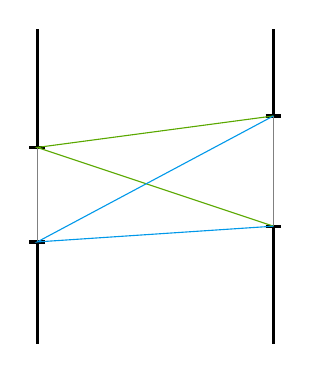
\begin{tikzpicture}[scale=1,%grid lines/.style={solid}
    ]
    \tikzmath{
      \h=2.0;
      \t=0.1;
      \zin=0;
      \ain=-0.7;
      \bin=+0.5;
      \zout=3;
      \aout=-0.5;
      \bout=+0.9;
    }
    \foreach \a/\b/\z/\l in {\ain/\bin/\zin/0, \aout/\bout/\zout/z} {
      \draw[very thick] (\z,\b) -- (\z,\h);
      \draw[very thick] (\z-\t,\b) -- (\z+\t,\b);
      \draw[very thick] (\z,\a) -- (\z,-\h);
      \draw[very thick] (\z-\t,\a) -- (\z+\t,\a);
      \draw[very thin, gray] (\z,\a) -- (\z,\b);
    }
    \draw[thin,draw=OwlGreen] (\zout,\bout) -- (\zin,\bin) -- (\zout,\aout);
    \draw[thin,draw=OwlBlue] (\zout,\bout) -- (\zin,\ain) -- (\zout,\aout);
  \end{tikzpicture}
  \caption{Propagation between two apertures.}
  \label{fig:propagation}
\end{figure}

In the considered conditions and assuming square supports to simplify, the
direct computation of the discrete convolution by
Eq.~\eqref{eq:discrete-convolution} takes about
$2\,L_{0}^{2}\,L_{z}^{2} \sim 2\,L^{4}$ operations with $L$ the typical value
of $L_{0}$ and $L_{z}$. Computation by fast Fourier transform (FFT) takes about
$3\,N^{2}\,\log_{2}N^{2} \sim 3\,(3\,L)^{2}\,\log_{2}((3\,L)^{2}) \sim 54\,L^{2}\,\log_{2}L$
operations. For large\footnote{not so large in fact, since the FFT-based method
  is faster for $L ≥ 10$ ignoring overheads} $L$'s, the FFT-based method is
much faster despite the larger size of the required grid.


\subsubsection{Sampling and range constraints in Rayleigh-Sommerfeld diffraction}
\label{sec:Rayleigh-Sommerfeld-diffraction:sampling-constraint}

The propagation kernel $h_{z}(\V{x})$ in Rayleigh-Sommerfeld diffraction is
given by Eq.~\eqref{eq:Rayleigh-Sommerfeld-kernel} and the most constraining
term for the sampling step is the phase of the $\mathe^{\mathi\,k\,r}$ term
since it varies by more than $π$ radians when the variation of $r$ between
adjacent samples is greater than $λ/2$.

In Rayleigh-Sommerfeld kernel $h_{z}(\V{x})$ given by
Eq.~\eqref{eq:Rayleigh-Sommerfeld-kernel}, the propagation distance is:
\begin{equation}
  \label{eq:r(x)}
  r(\V{x}) = \sqrt{\Norm*{\V{x}}^{2} + z^{2}}
\end{equation}
with $z > 0$ the distance along the optical axis between the input and output
transverse planes. To avoid irreversible phase wrapping, the phase difference
between two adjacent nodes of the sampling grid must not be greater than $π$
which yields the condition $k\,δr_{\Tag{max}} ≤ π$ or equivalently
$δr_{\Tag{max}} ≤ λ/2$ with $δr_{\Tag{max}}$ the greatest absolute variation of
$r$ between 2 adjacent nodes in the sampling grid:
\begin{equation}
  \label{eq:δr_max}
  δr_{\Tag{max}}
  = \max_{\substack{\V{x} ∈ Ω\\δ\V{x} ∈ δΩ}} \Abs*{r(\V{x} + δ\V{x}) - r(\V{x})}
\end{equation}
with $Ω = Ω_{z} - Ω_{0}$ the discrete kernel support accounting for all
differences in transverse positions between the input and output transverse
planes and:
\begin{equation}
  \label{eq:δΩ}
  δΩ = \Brace*{(±δx,0),(0,±δx)}
\end{equation}
the offsets to the closest sampled nodes (the blue dots in
Fig.~\ref{fig:closest-nodes}).

\begin{figure}
  \centering
  \begin{tikzpicture}[scale=1,%grid lines/.style={solid}
    ]
    \tikzmath{
      \R=1.2; % magnifier radius
      \r=0.15; % small disk radius
      \s=0.55; % magnified grid step
      \h=1.1*\r; % half-size of grid in caption
    }
    \draw[grid lines] (-1.6,-1.6) grid[step=0.2] (1.6,1.6);
    \begin{scope}[xshift=-5mm,yshift=6mm]
      \fill [color=textbg] (0,0) circle (\R);
      \begin{scope} % scope to clip
        \clip (0,0) circle (\R);
        \begin{scope}[xshift=-2mm,yshift=1mm] % scope to shift
          \draw[grid lines] (-3*\s,-3*\s) grid[step=\s] (3*\s,3*\s);
          \fill [color=OwlGreen] (0,0) circle (\r);
          \foreach \x/\y in {-\s/0, \s/0, 0/-\s, 0/+\s} {
            \fill [color=OwlBlue] (\x,\y) circle (\r);
          }
        \end{scope}
      \end{scope}
      \draw[thick] (0,0) circle (\R);
    \end{scope}
    \begin{scope}[xshift=+22mm,yshift=-4mm] % caption
      \draw [grid lines] (-\h,-\h) grid[step=2/3*\h] (\h,\h);
      \draw (\r,0) node[right]{$N× N$ grid};
      \fill [color=OwlGreen] (0,-\s) circle (\r);
      \draw (\r,-\s) node[right]{node at $\V{j}$};
      \fill [color=OwlBlue] (0,-2*\s) circle (\r);
      \draw (\r,-2*\s) node[right]{nodes at $\V{j} + δ\V{j}$};
    \end{scope}
  \end{tikzpicture}
  \caption{Closest nodes on a grid. In green, the considered node at index
    $δ\V{j}$; in blue, its closest neighbors at index $δ\V{j} + δ\V{j}$ with
    $δ\V{j} ∈ \Brace{(±1,0),(0,±1)}$.}
  \label{fig:closest-nodes}
\end{figure}

Since it is required that $δx$ be small enough to correctly sample the
variations of $r$, the following approximation can be made:
\begin{align}
  \label{eq:δr,approx}
  r(\V{x} + δ\V{x}) - r(\V{x})
  ≈ \Inner*{\frac{∂r(\V{x})}{∂\V{x}}}{δ\V{x}}
  = \frac{\Inner{\V{x}}{δ\V{x}}}{r(\V{x})}
\end{align}
where $\Inner{}{}$ denotes the inner (scalar) product. Hence:
\begin{align}
  \label{eq:δr_max,i}
  δr_{\Tag{max}}
  ≈ \max_{\substack{\V{x} ∈ Ω\\δ\V{x} ∈ δΩ}}
  \Abs*{\frac{\Inner{\V{x}}{δ\V{x}}}{r(\V{x})}}
  &= \max_{\V{x} ∈ Ω}
     \frac{\max_{δ\V{x} ∈ δΩ}\Abs*{\Inner{\V{x}}{δ\V{x}}}}{r(\V{x})}
\end{align}
From the definition of $δΩ$ in Eq.~\eqref{eq:δΩ}, the numerator in the last
above right-hand side can be simplified to:
\begin{equation}
  \label{eq:max<x,δx>}
  \max_{δ\V{x} ∈ δΩ}\Abs*{\Inner{\V{x}}{δ\V{x}}} = δx\,\Norm*{\V{x}}_{∞}
\end{equation}
with $\Norm*{\V{x}}_{∞} = \max\Paren*{\Abs*{x},\Abs*{y}}$ the infinite
norm of $\V{x} = (x,y)$ and then:
\begin{align}
  \label{eq:δr_max,ii}
  δr_{\Tag{max}}
  ≈ δx\,\max_{\V{x} ∈ Ω} \frac{\Norm*{\V{x}}_{∞}}{r(\V{x})}.
\end{align}
Clearly, the nodes that have a given $\Norm*{\V{x}}_{∞} = ℓ$ and yet
the least $r(\V{x})$ are those such that $\V{x} = (±ℓ,0)$ or
$\V{x} = (0,±ℓ)$, hence:
\begin{equation}
  \label{eq:δr_max,iii}
  δr_{\Tag{max}}
  ≈ δx\,\max_{\V{x} ∈ Ω}
     \frac{\Norm*{\V{x}}_{∞}}{\sqrt{\Norm*{\V{x}}_{∞}^{2} + z^{2}}}.
\end{equation}
Deriving the function:
\begin{equation}
  \label{eq:δr}
  δr(ℓ) = \frac{ℓ}{\sqrt{ℓ^{2} + z^{2}}}
\end{equation}
yields:
\begin{equation}
  \label{eq:δr'}
  δr'(ℓ) = \frac{z^{2}}{\Paren*{ℓ^{2} + z^{2}}^{3/2}}
\end{equation}
which is non-negative, hence $δr(ℓ)$ is increasing with $ℓ$. The maximal
value for $δr$ is thus found at
$ℓ_{\Tag{max}} = \max_{\V{x} ∈ Ω} \Norm*{\V{x}}_{∞} = D/2$ with $D$
the transverse size of $Ω$ and finally:
\begin{equation}
  \label{eq:δr_max,end}
  δr_{\Tag{max}} ≈ \frac{δx\,D/2}{\sqrt{z^{2} + (D/2)^{2}}}
  = \frac{δx/2}{\sqrt{(z/D)^{2} + 1/4}}.
\end{equation}

The sampling condition for the Rayleigh-Sommerfeld kernel, that is
$δr_{\Tag{max}} ≤ λ/2$, finally writes:
\begin{equation}
  \frac{δx}{\sqrt{(z/D)^{2} + 1/4}} ≤ λ.
\end{equation}
This condition may be expressed as an upper bound on the sampling step:
\begin{equation}
  \label{eq:Rayleigh-Sommerfeld-sampling-condition}
  δx ≤ δx_{\Tag{max}} = λ\,\sqrt{(z/D)^{2} + 1/4}
  ≈
  \begin{cases}
    λ/2 & \text{when $\Abs{z} \ll D$}\\
    \Abs{z}\,λ/D & \text{when $\Abs{z} \gg D$}\\
  \end{cases}
\end{equation}
with $D$ the transverse size of $Ω$. In the near field, that is for $z \ll D$,
the bound is the Shannon sampling step to correctly sample all propagating
waves which have spatial frequencies up to $1/λ$. In the far field, that is for
$z \gg D$, the bound is the propagation distance along the optical axis times
the angular diffraction limit $λ/D$ for an aperture of size $D$. Note that,
even though the angular spectrum $\FT{u}_{0}(\V{α})$ of the field in the input
transverse plane has a cutoff frequency much smaller than
$1/(2\,δx_{\Tag{max}})$, the constraint $δx ≤ δx_{\Tag{max}}$ still applies to
avoid undersampling the kernel before computing its discrete Fourier transform.
To benefit from a cutoff frequency of the angular spectrum, another method must
be considered where the propagation transfer function $\FT{h}_{z}(\V{α})$ is
directly sampled.

Looking at Eq.~\eqref{eq:Rayleigh-Sommerfeld-sampling-condition}, it is clear
that having the smallest possible $D$ is desirable to relax the constraint on
the smallness of the sampling step. Going back to the discussion about the
sizes of the supports, near Eq.~\eqref{eq:convolution-grid-size}, it can be
seen that the smallest possible support size to sample the propagation kernel
is $D = D_{0} + D_{z}$ where $D_{0} = L_{0}\,δx$ and $D_{z} = L_{z}\,δx$ are
the respective sizes of the supports of the field in the input and output
transverse planes.

For a chosen sampling step, the sampling condition in
Eq.~\eqref{eq:Rayleigh-Sommerfeld-sampling-condition} can be converted into a
minimal range condition to apply this propagation method:
\begin{equation}
  \label{eq:Rayleigh-Sommerfeld-range-condition}
  \Abs{z} ≥ D\,\sqrt{(δx/λ)^{2} - 1/4}
\end{equation}
provided $δx > λ/2$; otherwise, $\Abs{z}$ can be as small as a few
wavelengths\footnote{if $\Abs{z}$ is less than a few $λ$, evanescent waves must
  be taken into account}. Again, to relax as much as possible this constraint,
$D$ must be as small as possible.

Remember that Rayleigh-Sommerfeld diffraction integral assumes $z ≥ 0$, that is
forward propagation, \textbf{reverse propagation} can nevertheless be
implemented as the deconvolution by the forward propagation kernel. \oops{Give
  the formal expression.}


\subsubsection{Sampling and range constraints for paraxial propagation kernel}

The paraxial (Fresnel) propagation kernel is given by
Eq.~\eqref{eq:Fresnel-kernel} which we recall for convenience:
\begin{equation}
  h_{z}(\V{x}) = \frac{\mathe^{\mathi\,k\,z}}{\mathi\,λ\,z}\,
  \mathe^{\mathi\,π\,\Norm*{\V{x}}^{2}/(λ\,z)}.
\end{equation}
Now the phase is varying as $ϕ(\V{x}) = π\,\Norm*{\V{x}}^{2}/(λ\,z)$ a
quadratic function of the transverse position $\V{x}$. The maximal absolute
difference of the quadratic phase between adjacent nodes of the grid is:
\begin{align}
  δϕ_{\Tag{max}}
  &= \max_{\substack{\V{x} ∈ Ω\\δ\V{x} ∈ δΩ}}
  \Abs*{ϕ(\V{x} + δ\V{x}) - ϕ(\V{x})} \\
  &= \frac{π}{λ\,\Abs{z}}\,
  \max_{\substack{\V{x} ∈ Ω\\δ\V{x} ∈ δΩ}}
  \Abs*{\Norm*{\V{x} + δ\V{x}}^{2} - \Norm*{\V{x}}^{2}}
\end{align}
with, as in the previous subsection, $Ω = Ω_{0} - Ω_{z}$ the set of nodes for
which the kernel must be evaluated and $δΩ$ given in Eq.~\eqref{eq:δΩ} the
offsets to the adjacent nodes. To estimate $δϕ_{\Tag{max}}$, we compute:
\begin{align}
  \label{eq:max-quadratic-diff}
  \max_{\substack{\V{x} ∈ Ω\\δ\V{x} ∈ δΩ}}
  \Abs*{\Norm*{\V{x} + δ\V{x}}^{2} - \Norm*{\V{x}}^{2}}
  &= \max_{\substack{\V{x} ∈ Ω\\δ\V{x} ∈ δΩ}}
  \Abs*{\Norm*{δ\V{x}}^{2} + 2\,\Inner{\V{x}}{δ\V{x}}}\\
  \label{eq:max-quadratic-diff,a}
  &= \max_{\substack{\V{x} ∈ Ω\\δ\V{x} ∈ δΩ}}
  \Abs*{δx^{2} + 2\,\Inner{\V{x}}{δ\V{x}}}\\
  &= δx^{2} + 2\,\max_{\substack{\V{x} ∈ Ω\\δ\V{x} ∈ δΩ}}
  \Abs*{\Inner{\V{x}}{δ\V{x}}}\\
  \label{eq:max-quadratic-diff,b}
  &= δx^{2} + 2\,δx\,\max_{\V{x} ∈ Ω}\Norm*{\V{x}}_{∞}\\
  \label{eq:max-quadratic-diff,c}
  &= δx^{2} + δx\,D
\end{align}
where right-hand side~\eqref{eq:max-quadratic-diff,a} follows from
$\Norm*{δ\V{x}} = δx$ for any $δ\V{x} ∈ δΩ$ with $δΩ$ defined in
Eq.~\eqref{eq:δΩ}, right-hand side~\eqref{eq:max-quadratic-diff,b} follows from
Eq.~\eqref{eq:max<x,δx>}, and right-hand side~\eqref{eq:max-quadratic-diff,c}
follows from $\max_{\V{x} ∈ Ω}\Norm*{\V{x}}_{∞} = D/2$ with $D$ the
transverse size of $Ω$. Note that, contrarily to the computations in
Eq.~\eqref{eq:δr,approx}, there are no approximations here. The maximal
absolute difference of the quadratic phase
\begin{equation}
  \label{eq:max-quadratic-diff}
  δϕ_{\Tag{max}}
  = \max_{\substack{\V{x} ∈ Ω\\δ\V{x} ∈ δΩ}}
  \Abs*{ϕ(\V{x} + δ\V{x}) - ϕ(\V{x})}
  = \frac{π\,(D + δx)\,δx}{λ\,\Abs{z}}
  ≈ \frac{π\,D\,δx}{λ\,\Abs{z}},
\end{equation}
the latter approximation since $D \gg δx$ in general. The condition
$δϕ_{\Tag{max}} ≤ π$ amounts to:
\begin{equation}
  \label{eq:}
  \frac{D\,δx}{λ\,\Abs{z}} ≤ 1
\end{equation}
which may be seen as an upper bound for the sampling step:
\begin{equation}
  \label{eq:paraxial-sampling-condition}
  δx ≤ \Abs{z}\,λ/D,
\end{equation}
or as a minimal propagation range condition:
\begin{equation}
  \label{eq:paraxial-range-condition}
  \Abs{z} ≥ D\,δx/λ.
\end{equation}
Compared to Eq.~\eqref{eq:Rayleigh-Sommerfeld-sampling-condition},
Eq.~\eqref{eq:paraxial-sampling-condition} corresponds to the far field case
$\Abs{z} \gg D$; while, compared to
Eq.~\eqref{eq:Rayleigh-Sommerfeld-range-condition},
Eq.~\eqref{eq:paraxial-range-condition} corresponds to $δx \gg λ/2$.

Note that the paraxial approximation of the propagation kernel assumes that the
condition in Eq.~\eqref{eq:paraxial-condition} holds which is equivalent to:
\begin{equation}
  \label{eq:paraxial-condition-for-z}
  \Abs{z} \gg \Paren*{\frac{\Norm*{\V{x}}^{4}}{8\,λ}}^{1/3}
\end{equation}
although \citet{Southwell.1981.Fresnel_approximation_validity} has shown that,
in practice, the Fresnel approximation works quite well for propagation
distances much smaller than that.

\subsection{Angular spectrum propagation}
\label{sec:angular_spectrum_propagation}

The angular spectrum propagation method is similar to the propagation by
convolution computed by means of FFT's, the only difference is that the
propagation transfer function $\FT{h}_{z}(\V{α})$ is directly sampled instead
of being given by a DFT of the sampled propagation kernel $h_{z}(\V{x})$. This
numerical approximation of the optical propagation writes:
\begin{align}
  \V{u}_{z}
  &= \Paren*{δα^{2}\,\M{F}^{\star}}·
    \Diag\Paren*{\FT{\V{h}}_{z}}·
    \Paren*{δx^{2}\,\M{F}}· \V{u}_{0}\notag\\
  &= \underbrace{
    \frac{1}{N^{2}}·\M{F}^{\star}·
    \Diag\Paren*{\FT{\V{h}}_{z}}·\M{F}
    }_{\text{propagator}}· \V{u}_{0}
    \label{eq:numerical-angular-spectrum-propagation}
\end{align}
since $δx\,δα = 1/N$ for the approximation of the Fourier transform by the DFT
operator $\M{F}$ and with $\Diag(\FT{\V{h}}_{z})$ the linear operator
implementing element-wise multiplication by $\FT{\V{h}}_{z}$ the propagation
transfer function sampled at discrete frequencies $\V{α}[\V{j}] = δα\,\V{j}$.

The first condition that must hold to apply this method is that the Nyquist
frequency for a $N× N$ grid of discrete spatial frequencies:
\begin{equation}
  \label{eq:Nyquist-frequency}
  \NyquistFreq = (N/2)\,δα = \frac{1}{2\,δx}
\end{equation}
must not be smaller than the cutoff frequency $\CutoffFreq$ of the input
angular spectrum:
\begin{equation}
  \label{eq:cutoff-constraint}
  \NyquistFreq ≥ \CutoffFreq
  \quad\Longrightarrow\quad
  δx ≤ \frac{1}{2\,\CutoffFreq}
\end{equation}
\oops{Note that, taking the intensity, that is the squared modulus of the
  complex amplitude, effectively doubles the cutoff frequency.}

As before but in the frequency space, another condition to approximate the
integral over frequencies for the final Fourier transform by a Riemann sum is
that the frequency sampling step $δα$ be fine enough to correctly sample the
variation of the propagation transfer function $\FT{h}_{z}(\V{α})$. This
depends on the considered case, non-paraxial or paraxial as examined next.


\subsection{Angular spectrum frequencies}
\label{sec:angular_spectrum_frequencies}

The diffraction integral states that, when propagating from $\V{r}' ∈ Σ$ to
$\V{r}$, the phase of the field becomes:
\begin{equation}
  \label{eq:phase_transfer}
  ϕ(\V{r},\V{r}') = φ_{z'}(\V{x}') + ψ(\V{r},\V{r}')
\end{equation}
where $φ_{z'}(\V{x}')$ is the phase of the wavefront leaving the input
transverse plane at $z'$ while
$ψ_{z - z'}(\V{x} - \V{x}') = \Arg\Paren*{h_{z - z'}(\V{x} - \V{x}')}$ is the
phase shift due to the propagation kernel. The phase $φ_{z'}(\V{x}')$ is
introduced for generality, it may account for the phase of the complex
amplitude transmission of the aperture in the input transverse plane, for a
quadratic phase term due to a thin lens or to the Fresnel transform in the
paraxial conditions, etc.

The variation of the phase $ϕ(\V{r},\V{r}')$ in the input transverse plane can
be interpreted as the transverse wave-vector $\V{k}_{\perp}$ of a planar wave
propagating from $\V{r}'$ to $\V{r}$:
\begin{equation}
  \V{k}_{\perp}(\V{r},\V{r}') = \frac{\partial ϕ(\V{r},\V{r}')}{\partial \V{x}'}
\end{equation}
which corresponds, see Eq.~\eqref{eq:spatial-frequencies}, to the angular
spectrum frequency:
\begin{equation}
  \label{eq:propagating_frequency}
  \V{α}(\V{r},\V{r}') = \frac{\V{k}_{\perp}(\V{r},\V{r}')}{2\,π}
  = \frac{1}{2\,π}\,\frac{\partial ϕ(\V{r},\V{r}')}{\partial \V{x}'}.
\end{equation}
Now if the field $u_{z'}(\V{x}')$ in the input transverse plane at $z'$ has a
finite size support\footnote{The support of a function contains all arguments
  where the function is non-zero.} $Ω' \subset Σ$ and if we only need to
estimate the field $u_{z}(\V{x})$ over a finite size subset, $Ω$, of the output
transverse plane at $z$, the angular spectrum propagation can be restricted to
the frequencies $\V{α} \in Ξ$ with $Ξ$ the set of propagating frequencies
defined by:
\begin{equation}
  \label{eq:propagating_frequencies}
  Ξ = \Brace*{
    \V{α}(\V{r},\V{r}') \Given
    \V{r} \in Ω
    \text{\ and\ }
    \V{r}' \in Ω'
  }
\end{equation}
where $\V{α}(\V{r},\V{r}')$ is defined in Eq.~\eqref{eq:propagating_frequency}.
Note that $Ξ$ is finite following from $Ω'$ and $Ω'$ being both finite. Having
a finite range of frequencies to consider is crucial to limit the numerical
complexity of performing the propagation by the angular spectrum method.

% \begin{cases}
%   k\,\Norm*{\V{r} - \V{r}'} & \text{in the non-paraxial case}\\
%   k\,(z - z') + k\,\dfrac{\Norm*{\V{x} - \V{x}'}^{2}}{2\,(z - z')} & \text{in the paraxial case}\\
% \end{cases}

\subsubsection{Propagation by the non-paraxial transfer function}

The non-paraxial transfer function given in
Eq.~\eqref{eq:propagation-transfer-function} is:
\begin{equation}
  \FT{h}_{z}(\V{α}) = \mathe^{\mathi\,k\,z\,\sqrt{1 - \Norm*{λ\,\V{α}}^{2}}}.
\end{equation}
Evanescent waves whose frequencies are greater than $1/λ$ are rapidly vanishing
and negligible for $\Abs{z}$ greater or equal a few wavelengths. Hence, we
shall only consider propagating waves, that is spatial frequencies such that
$\Norm*{\V{α}} < 1/λ$. For these frequencies, the variations of the phase
\begin{equation}
  \label{eq:non-paraxial_transfer_function_phase}
  ϕ(\V{α}) = k\,z\,\sqrt{1 - \Norm*{λ\,\V{α}}^{2}}
\end{equation}
of the transfer function between contiguous discrete frequencies must not be
greater than $π$ which imposes that:
\begin{equation}
  \label{eq:non-paraxial_phase_variation_condition}
  \Abs*{ϕ(\V{α} + δ\V{α}) - ϕ(\V{α})} ≤ π
\end{equation}
must hold for any $\V{α} ∈ Ξ$ and any $δ\V{α} ∈ δΞ$ with:
\begin{equation}
  δΞ = \Brace*{(±δα,0),(0,±δα)}
\end{equation}
the offsets to contiguous spatial frequencies (the blue dots in
Fig.~\ref{fig:closest-nodes}) and with:
\begin{equation}
  Ξ = \Brace*{
    \V{α} ∈ \Set{R}^{2} \Given
    \Norm{\V{α}}_{∞} ≤ \NyquistFreq
    \text{\ and\ }
    \Norm{\V{α}} < \min(\CutoffFreq,1/λ)
  }\\
\end{equation}
the domain of spatial frequencies to consider with $\NyquistFreq$ the Nyquist
frequency defined in Eq.~\eqref{eq:Nyquist-frequency} and
$\min(\CutoffFreq,1/λ)$ the maximal frequency of waves existing in the input
angular spectrum and that can propagate.

Assuming the spectral sampling step $δα = 1/(N\,δx)$ is small enough, the
maximal absolute phase difference can be estimated following the same steps as
in section~\ref{sec:Rayleigh-Sommerfeld-diffraction:sampling-constraint}:
\begin{align}
  δϕ_{\Tag{max}}
  &=\max_{\substack{\V{α} ∈ Ξ\\δ\V{α} ∈ δΞ}}
  \Abs*{ϕ(\V{α} + δ\V{α}) - ϕ(\V{α})} \\
  &\simeq \max_{\substack{\V{α} ∈ Ξ\\δ\V{α} ∈ δΞ}}
  \Abs*{\Inner*{\frac{∂ϕ(\V{α})}{∂\V{α}}}{δ\V{α}}}\\
  &= 2\,π\,\Abs*{z}\,λ\,\max_{\substack{\V{α} ∈ Ξ\\δ\V{α} ∈ δΞ}}
  \Abs*{\frac{\Inner*{\V{α}}{δ\V{α}}}{\sqrt{1 - \Norm{λ\,\V{α}}^{2}}}}\\
  &= 2\,π\,\Abs*{z}\,λ\,\max_{\V{α} ∈ Ξ}
    \frac{\max_{δ\V{α} ∈ δΞ}\Abs*{\Inner*{\V{α}}{δ\V{α}}}}
    {\Abs*{\sqrt{1 - \Norm{λ\,\V{α}}^{2}}}}\\
  &= 2\,π\,\Abs*{z}\,λ\,δα\,\max_{\V{α} ∈ Ξ}
    \frac{\Norm*{\V{α}}_{∞}}
    {\Abs*{\sqrt{1 - \Norm{λ\,\V{α}}^{2}}}}.
    \label{eq:δϕ_max:nonparaxial}
\end{align}
If
$\max_{\V{α} ∈ Ξ}\Norm{\V{α}} = \min(\CutoffFreq,\sqrt{2}\,\NyquistFreq) ≥ 1/λ$,
then $\sqrt{1 - \Norm{λ\,\V{α}}^{2}}$ may be arbitrarily close to zero for
$\Norm*{\V{α}}_{∞} > 0$. Hence, the condition in
Eq.~\eqref{eq:non-paraxial_phase_variation_condition} cannot hold and phase
wrapping is irreversible. Otherwise, maximizing the right-hand-side in
Eq.~\eqref{eq:δϕ_max:nonparaxial} amounts to finding the frequencies in $Ξ$
such that $\Norm*{\V{α}}_{∞}$ and $\Norm*{\V{α}}$ are both maximized. The
3 possibilities are illustrated by
Fig.~\ref{fig:phase-wrapping-non-paraxial-transfer}. If
$\sqrt{2}\,\NyquistFreq < \min(1/λ,\CutoffFreq)$, then the worst spatial
frequencies are indicated by blue dots in the leftmost panel of
Fig.~\ref{fig:phase-wrapping-non-paraxial-transfer} and:
\begin{equation}
  \max_{\V{α} ∈ Ξ} \frac{\Norm*{\V{α}}_{∞}}
  {\Abs*{\sqrt{1 - \Norm{λ\,\V{α}}^{2}}}}
  = \frac{\NyquistFreq}{\sqrt{1 - 2\,λ^{2}\,\NyquistFreq^{2}}};
\end{equation}
else if $\NyquistFreq ≤ \CutoffFreq < 1/λ$, then the worst
spatial frequencies are indicated by green dots in the central panel of
Fig.~\ref{fig:phase-wrapping-non-paraxial-transfer} and:
\begin{equation}
  \max_{\V{α} ∈ Ξ} \frac{\Norm*{\V{α}}_{∞}}
  {\Abs*{\sqrt{1 - \Norm{λ\,\V{α}}^{2}}}}
  = \frac{\NyquistFreq}{\sqrt{1 - λ^{2}\,\CutoffFreq^{2}}};
\end{equation}
finally, if $\CutoffFreq < \min(1/λ,\NyquistFreq)$, then the worst
spatial frequencies are indicated by orange dots in the rightmost panel
of Fig.~\ref{fig:phase-wrapping-non-paraxial-transfer} and:
\begin{equation}
  \label{eq:max-term:3rd-case:nonparaxial}
  \max_{\V{α} ∈ Ξ} \frac{\Norm*{\V{α}}_{∞}}
  {\Abs*{\sqrt{1 - \Norm{λ\,\V{α}}^{2}}}}
  = \frac{\CutoffFreq}{\sqrt{1 - λ^{2}\,\CutoffFreq^{2}}}.
\end{equation}
Combining these 3 possibilities:
\begin{equation}
  \max_{\V{α} ∈ Ξ} \frac{\Norm*{\V{α}}_{∞}}
  {\Abs*{\sqrt{1 - \Norm{λ\,\V{α}}^{2}}}}
  = \frac{\min(\CutoffFreq,\NyquistFreq)}{\sqrt{1 - λ^{2}\,\min(\CutoffFreq,\sqrt{2}\,\NyquistFreq)^{2}}}.
\end{equation}
In principle, to avoid aliasing, the sampling step must be chosen so that the
Nyquist frequency is not less than the cutoff frequency, that is
$\NyquistFreq ≥ \CutoffFreq$, so that the above right-hand side is given by
Eq.~\eqref{eq:max-term:3rd-case:nonparaxial}. In this case the sampling
conditions are:
\begin{equation}
  \label{eq:nonparaxial-angular-spectrum-sampling-conditions}
  \begin{cases}
    \displaystyle
    \frac{2\,λ\,\CutoffFreq\,\Abs*{z}\,δα}{\sqrt{1 - λ^{2}\,\CutoffFreq^{2}}}
    =\frac{2\,λ\,\CutoffFreq\,\Abs*{z}}{N\,δx\,\sqrt{1 - λ^{2}\,\CutoffFreq^{2}}}
    ≤ 1\\[2ex]
    \displaystyle
    δx ≤ \frac{1}{2\,\CutoffFreq}
  \end{cases}
\end{equation}
which can be combined in a bracketing condition for the sampling step $δx$:
\begin{equation}
  \label{eq:nonparaxial-angular-spectrum-sampling-bracketing}
  \frac{2\,λ\,\Abs*{z}\,\CutoffFreq}{N\,\sqrt{1 - λ^{2}\,\CutoffFreq^{2}}}
  ≤ δx ≤ \frac{1}{2\,\CutoffFreq}.
\end{equation}


\begin{figure}
  \centering
  \begin{tikzpicture}[scale=1,%grid lines/.style={solid}
    ]
    \tikzmath{
      \xshift=1;
      \r=0.1; % small disk radius
      \gridsize=1.2;
      \gridradius=\gridsize/sqrt(2);
      \smallstep=0.05*\gridsize;
      \Ar=1.2*\gridradius;
      \Ax=\gridsize/2;
      \Ay=\Ax;
      \Br=0.85*\gridradius; % med. radius
      \Bx=\Ax;
      \By=sqrt(\Br^2 - \Bx^2);
      \Cr=0.45*\gridradius; % min. radius
    }
    % Case A:
    \begin{scope}[xshift=-30mm]
      \fill[fill=gray!20] (-\Ax,-\Ay) rectangle (\Ax,\Ay);
      \foreach \x in {-\Ax,+\Ax} {
        \foreach \y in {-\Ax,+\Ax} {
          \fill [color=OwlBlue] (\x,\y) circle (\r);
        }
      }
      \draw (-\Ax,-\Ay) rectangle (\Ax,\Ay);
      \draw (0,0) circle (\Ar);
      \draw[<-] (60:\Ar) -- (60:\Ar+0.4) -- ++(0.4,0) node [anchor=west] {$\CutoffFreq$};
    \end{scope}
    % Case B:
    \begin{scope}
      \fill[fill=gray!20] (-\Ax,-\Ay) rectangle (\Ax,\Ay);
      \foreach \x in {-\Bx,+\Bx} {
        \foreach \y in {-\By,+\By} {
          \fill [color=OwlGreen] (\x,\y) circle (\r);
          \fill [color=OwlGreen] (\y,\x) circle (\r);
        }
      }
      \draw (-\Ax,-\Ay) rectangle (\Ax,\Ay);
      \draw (0,0) circle (\Br);
    \end{scope}
   % Case C:
     \begin{scope}[xshift=25mm]
      \fill[fill=gray!20,draw=textfg] (-\Ax,-\Ay) rectangle (\Ax,\Ay);
      \foreach \x/\y in {0/-\Cr, +\Cr/0, 0/+\Cr, -\Cr/0} {
        \fill [color=OwlOrange] (\x,\y) circle (\r);
        \fill [color=OwlOrange] (\y,\x) circle (\r);
      }
      \draw (0,0) circle (\Cr);
      \tikzmath{\tick=0.15; \x = \Ax + 2*\tick;}
      \draw[->] (\x, -\Ay - 0.5*\tick) -- (\x, \Ay + 2*\tick);
      \foreach \y in {-\Ay,0,\Ay} {
        \draw (\x, \y) -- (\x + \tick, \y);
      }
      \draw (\x + 0.7*\tick, -\Ay) node [anchor=west] {$-\NyquistFreq$};
      \draw (\x + 0.7*\tick,    0) node [anchor=west] {$0$};
      \draw (\x + 0.7*\tick, +\Ay) node [anchor=west] {$+\NyquistFreq$};
    \end{scope}
  \end{tikzpicture}
  \caption{Spatial frequencies (indicated by colored circles) where the phase
    wrapping is the most severe for the non-paraxial propagation transfer
    function. For the 3 possible cases, the grayed square indicates the area
    sampled by the DFT with $\NyquistFreq$ the Nyquist frequency, and the
    circle indicates the cutoff frequency $\CutoffFreq$ of the angular spectrum
    assumed to be less the evanescent waves limit at $1/λ$.}
  \label{fig:phase-wrapping-non-paraxial-transfer}
\end{figure}


\subsubsection{Propagation by the paraxial transfer function}

In the paraxial conditions, the propagation transfer function is given by
Eq.~\eqref{eq:paraxial-transfer-function} which corresponds to frequencies much
smaller than $1/λ$:
\begin{equation}
  \FT{h}_{z}(\V{α}) \underset{\Norm*{\V{α}} \ll 1/λ}{≈}
  \mathe^{\mathi\,k\,z}\,
  \mathe^{-\mathi\,π\,λ\,z\,\Norm*{\V{α}}^{2}}.
\end{equation}

The worst frequencies for the quadratic phase term
$ϕ(\V{α}) = π\,λ\,z\,\Norm*{\V{α}}^{2}$ are such
\begin{align}
  δϕ_{\Tag{max}}
  &=\max_{\substack{\V{α} ∈ Ξ\\δ\V{α} ∈ δΞ}}
  \Abs*{ϕ(\V{α} + δ\V{α}) - ϕ(\V{α})} \\
  &= π\,λ\,\Abs*{z}\,\max_{\substack{\V{α} ∈ Ξ\\δ\V{α} ∈ δΞ}}
  \Abs*{\Norm*{\V{α} + δ\V{α}}^{2} - \Norm*{\V{α}}^{2}}\\
  &= π\,λ\,\Abs*{z}\,\max_{\substack{\V{α} ∈ Ξ\\δ\V{α} ∈ δΞ}}
  \Abs*{\Norm*{δ\V{α}}^{2} + 2\,\Inner{\V{α}}{δ\V{α}}}\\
  &= π\,λ\,\Abs*{z}\,\Paren[\Big]{δα^{2} + 2\,δα\,\max_{\V{α} ∈ Ξ}\Norm*{\V{α}}_{∞}}\\
  &≈ 2\,π\,λ\,\Abs*{z}\,δα\,\max_{\V{α} ∈ Ξ}\Norm*{\V{α}}_{∞}\\
  &= 2\,π\,λ\,\Abs*{z}\,δα\,\min\Paren{\NyquistFreq,\CutoffFreq,1/λ}
\end{align}
which (as expected) correspond to the conditions in Eq.~\eqref{eq:nonparaxial-angular-spectrum-sampling-conditions} at low-frequencies.

\begin{equation}
  \label{eq:2}
  \begin{cases}
    \displaystyle
    \CutoffFreq \ll 1/λ\\[1ex]
    \displaystyle
    \CutoffFreq ≤ \NyquistFreq\\[1ex]
    \displaystyle
    2\,λ\,\CutoffFreq\,\Abs*{z}\,δα = \frac{2\,λ\,\CutoffFreq\,\Abs*{z}}{N\,δx} ≤ 1
  \end{cases}
\end{equation}

\subsection{Propagation by the Fresnel transform}


\subsection{Discrete computations}

See \citet{Sziklas-1974-diffraction_calculations} and \citet{Sziklas-1975-FFT_method}.

Several methods have been proposed for the numerical propagation of
2-dimensional sampled planar fields of size $N×N$. Discrete approximation by
a Riemann sum of the diffraction integral equation requires
$\mathcal{O}(N^{4})$ numerical floating-point operations, finite difference
methods to numerically solve the differential Helmholtz equation is as
demanding because of the number of steps to propagate the wave
\citep{Sziklas-1975-FFT_method}. Using the Fast Fourier Transform (FFT) to
compute the convolution product (the so-called angular spectrum method)
requires $\mathcal{O}(N^{2}\,\log_{2}N)$ operations but imposes that the
sampling steps $δx$ in the transverse planes be the same along the propagation.

\paragraph{Angular spectrum propagation.}
In this method, the propagation between a transverse plane at $z_{0}$ to a
transverse plane at $z_{1} = z_{0} + Δz$ is implemented by a discrete
convolution of the field $u_{z_{0}}$ by the shift-invariant propagation kernel
$h_{Δz}$. For speed, the discrete convolution is computed by means of Fast
Fourier Transforms (FFTs).

The sampled angular spectrum is given by:
\begin{align}
  \label{eq:angular-spectrum-dicretization}
  \FT{\boldsymbol{u}}_{z}[ℓ_{1},ℓ_{2}]
  &= \FT{u}_{z}(α_{x}[ℓ_{1}],α_{y}[ℓ_{2}])\notag\\
  &= \iint u_{z}(x,y)\,\mathe^{-\mathi\,2\,π\,(α_{x}[ℓ_{1}]\,x,α_{y}[ℓ_{2}]\,y)}
    \mathd x\, \mathd y\notag\\
  &≈ \sum_{k_{1},k_{2}} u_{z}(x[j_{1}],y[j_{2}])\,
    \mathe^{-\mathi\,2\,π\,(α_{x}[ℓ_{1}]\,x[j_{1}],α_{y}[ℓ_{2}]\,y[j_{2}])}\,
    |δx\,δy|\notag\\
  &= |δx\,δy|\,\bigl(\mathbf{F}·\boldsymbol{u}_{z}\bigr)[ℓ_{1},ℓ_{2}]
\end{align}
where $\mathbf{F}$ is the forward DFT operator (see Appendix~\ref{sec:DFT}),
$\boldsymbol{u}_{z}$ is the sampled field $u_{z}(x,y)$ with sampling step sizes
$δx$ and $δy$ along the $x$ and $y$ dimensions, and the square brackets are
used to index the sampled quantities (as in the first line of the above
equation). According to the properties of the DFT, the discrete angular
spectrum $\FT{\boldsymbol{u}}_{z}$ is sampled with steps $δα_{x}=1/(N_{1}\,δx)$ and
$δα_{y}=1/(N_{2}\,δy)$. In the following, we assume that the sampling steps and the
number of samples are the same along the two transverse Cartesian axes so that:
$N_{1} = N_{2} = N$ and $δx = δy$ and thus:
\begin{equation}
  \label{eq:discrete-angular-spectrum}
  \FT{\boldsymbol{u}}_{z} = |δx|^{2}\,\mathbf{F}·\boldsymbol{u}_{z},
\end{equation}
is the discrete angular spectrum with frequency sampling steps
$δα_{x} = δα_{y} = 1/(N\,δx)$. Conversely:
\begin{equation}
  \label{eq:inverse-discrete-angular-spectrum}
  \boldsymbol{u}_{z} = |δα|^{2}\,\mathbf{F}^{\star}·\FT{\boldsymbol{u}}_{z},
\end{equation}
where $\mathbf{F}^{\star}$, the adjoint of $\mathbf{F}$, is the backward DFT
operator. It is easy to check that
Eq.~\eqref{eq:inverse-discrete-angular-spectrum} with
$δα = 1/(N\,δx)$ is indeed the inverse of
Eq.~\eqref{eq:discrete-angular-spectrum}:
\begin{displaymath}
  |δα|^{2}\,\mathbf{F}^{\star}·\FT{\boldsymbol{u}}_{z}
  = \frac{1}{(N\,|δx|)^{2}}\,\mathbf{F}^{\star}·\Paren*{|δx|^{2}\,\mathbf{F}·\boldsymbol{u}_{z}} = \frac{1}{N^{2}}\,\mathbf{F}^{\star}·\mathbf{F}·\boldsymbol{u}_{z}
  = \boldsymbol{u}_{z}
\end{displaymath}
where the last simplification follows from Eq.~\eqref{eq:inverse-DFT-operator}.
The field in the transverse plane at $z_{1}$ knowing the field in the
transverse plane at $z_{0}$ is given by:
\begin{equation}
  \label{eq:7}
  \boldsymbol{u}_{z_{1}} = \frac{1}{N^{2}}\,\mathbf{F}^{\star}·
  \mathrm{diag}\bigl(\FT{\boldsymbol{h}}_{z_{1} - z_{0}}\bigr)·
  \mathbf{F}·\boldsymbol{u}_{z_{0}}
\end{equation}
where $\mathrm{diag}(\boldsymbol{a})$ denotes a diagonal linear operator whose
diagonal entries are those of $\boldsymbol{a}$ and such that applying this
operator to, say, $\boldsymbol{b}$ yields the element-wise multiplication of
$\boldsymbol{a}$ and $\boldsymbol{b}$. In the above equation,
$\FT{\boldsymbol{h}}_{z_{1} - z_{0}}$ is either the discrete Fourier transform,
as defined in Eq.~\eqref{eq:discrete-angular-spectrum}, of the propagation
kernel $h_{z_{1} - z_{0}}(x,y)$ sampled with steps of size $δx$ or
$\FT{h}_{z_{1} - z_{0}}(\V{α})$ sampled with steps of size $δα = 1/(N\,δx)$.
Due to the approximation of the continuous Fourier transform by the discrete
transform, the two are not exactly equivalent.

The operator implementing the propagation by means of the angular spectrum
writes:
\begin{equation}
  \label{eq:angular-spectrum-propagator}
  \mathbf{H}_{z}^{\text{conv}} = \frac{1}{N^{2}}\,\mathbf{F}^{\star}·
  \mathrm{diag}\bigl(\FT{\boldsymbol{h}}_{z}\bigr)·
  \mathbf{F}.
\end{equation}
With this method, the sampling steps are unchanged and the exact or paraxial
planar propagation may be modeled. The methods considered next specifically
implement Fresnel diffraction that is assuming the paraxial approximation.

To avoid aliasing, $\mathcal{D}_{1/λ}$ must be inside the support sampled by
the discrete frequencies. Hence, the Nyquist frequency must not be smaller than
$1/λ$ which writes:
\begin{equation}
  \label{eq:no-aliasing-condition}
  (N/2)\,δα ≥ 1/λ
  \quad\Longleftrightarrow\quad
  δx ≤ λ/2.
\end{equation}

\paragraph{Single-FFT Fresnel propagation.}
\label{sec:single-FFT-Fresnel-propagation}
In the paraxial approximation (Fresnel diffraction), the propagation kernel is
given by Eq.~\eqref{eq:Fresnel-kernel} and the resulting field in transverse
plane at $z_{1} = z_{0} + Δz$ is:
\begin{align}
  u_{z_{1}}(\V{x}_{1})
  &= \iint u_{z_{0}}(\V{x}_{0})\,h_{Δz}(\V{x}_{1} - \V{x}_{0})\,
    \mathd\V{x}_{0} \notag\\
  &= \frac{\mathe^{\mathi\,k\,Δz}}{\mathi\,λ\,Δz}
    \iint u_{z_{0}}(\V{x}_{0})\,
    \mathe^{\mathi\,k\,\frac{\Norm*{\V{x}_{1} - \V{x}_{0}}^{2}}{2\,Δz}}\,
    \mathd\V{x}_{0} \notag\\
  &= \frac{\mathe^{\mathi\,k\,Δz}}{\mathi\,λ\,Δz}\,
    \mathe^{\mathi\,k\,\frac{\Norm*{\V{x}_{1}}^{2}}{2\,Δz}}\,
    \iint \Brack*{
    u_{z_{0}}(\V{x}_{0})\,
    \mathe^{\mathi\,k\,\frac{\Norm*{\V{x}_{0}}^{2}}{2\,Δz}}
    }\,
    \mathe^{-\mathi\,k\,\frac{\Inner{\V{x}_{1}}{\V{x}_{0}}}{Δz}}\,
    \mathd\V{x}_{0}
\end{align}
where the integral in the last right-hand side is similar to taking the Fourier
transform of the term in square brackets. This integral can thus be computed by
a single DFT provided the sampling condition in
Eq.~\eqref{eq:DFT-sampling-condition,nD} holds which imposes that:
\begin{equation}
  \label{eq:9}
  \frac{k\,δx_{0}\,δx_{1}}{Δz} = ±\frac{2\,π}{N}
\end{equation}
with $N$ the number of samples along a transverse dimension. The sampling step
in the output plane is thus given by:
\begin{equation}
  \label{eq:one-step-sampling-rule}
  δx_{1} = \frac{λ\,\Abs*{Δz}}{N\,δx_{0}}
\end{equation}
and the double integral is approximated by $δx_{0}^{2}\,\M{F}$ if $Δz > 0$ and
by $δx_{0}^{2}\,\M{F}^{\star}$ if $Δz < 0$ with $\M{F}$ the 2-dimensional
discrete Fourier transform operator (see Appendix~\ref{sec:DFT}). Note that,
with this latter convention, the transverse axes ($x$ and $y$) keep their
orientation.

Using bold lowercase symbols to represent sampled quantities and bold uppercase
symbols to represent operators, \textbf{single-FFT Fresnel propagation} writes:
\begin{equation}
  \label{eq:single-FFT-Fresnel-propagation}
  \tcboxmath{
    \begin{array}{l}
      \displaystyle
      \V{u}_{z_{1}} = \frac{δx_{0}^{2}\,\mathe^{\mathi\,k\,Δz}}{\mathi\,λ\,Δz}\,
      \M{Q}_{\frac{δx_{1}^{2}}{λ\,Δz}}·
      \M{F}_{Δz}·
      \M{Q}_{\frac{δx_{0}^{2}}{λ\,Δz}}·
      \V{u}_{z_{0}}\\[2ex]
      \displaystyle
      δx_{1} = \frac{λ\,\Abs*{Δz}}{N\,δx_{0}}\\[2ex]
      \displaystyle
      Δz = z_{1} - z_{0}\\[2ex]
      \displaystyle
      \M{F}_{Δz} =
      \begin{cases}
        \M{F} & \text{if $Δz > 0$,}\\
        \M{F}^{\star} & \text{if $Δz < 0$}
      \end{cases}
      \\[2ex]
      \displaystyle
      \M{Q}_{ρ} = \Diag\Paren*{\V{q}_{ρ}}
      \quad\text{with}\quad
      \V{q}_{ρ}[\V{j}] =
      \mathe^{\mathi\,π\,ρ\,\Norm*{\V{j}}^{2}}
      \quad ∀ \V{j} ∈ \Set{J}×\Set{J}
    \end{array}
  }
\end{equation}
where operator $\M{F}_{Δz}$ is to simplify the notation while operator
$\M{Q}_{ρ}$ implements element-wise multiplication by a quadratic phase factor.
Note that multiplication by the scalar $δx_{0}^{2}$ commutes with all operators
but that operators $\M{F}_{Δz}$ and $\M{Q}_ρ$ do not commute. Also note that
$\V{u}_{z_{0}}$ and $\V{u}_{z_{1}}$ denote the complex amplitude in the
transverse planes respectively at $z_{0}$ and $z_{1}$ and respectively sampled
with steps $δx_{0}$ and $δx_{1}$ which are related by
Eq.~\eqref{eq:one-step-sampling-rule} and are usually not equal.

%\begin{equation}
%  \label{eq:directed-DFT}
%  \M{F}_{Δz} =
%  \begin{cases}
%    \M{F} & \text{if $Δz > 0$,}\\
%    \M{F}^{\star} & \text{if $Δz < 0$}
%  \end{cases}
%\end{equation}
%\begin{equation}
%  \label{eq:quadratic-phase-operator}
%  \M{Q}_{ρ} = \Diag\Paren*{\V{q}_{ρ}}
%  \quad\text{with}\quad
%  \V{q}_{ρ}[\V{j}] =
%  \mathe^{\mathi\,π\,ρ\,\Norm*{\V{j}}^{2}}
%  \quad∀ \V{j} ∈ \Set{J}×\Set{J}
%\end{equation}

In continuous coordinates, the quadratic phase factors is given by:
\begin{equation}
  \label{eq:quadratic-phase-factor}
  \mathcal{Q}_{ρ}\Paren*{\V{x}} = \mathe^{\mathi\,π\,ρ\,\Norm*{\V{x}}^{2}},
\end{equation}
whose 2-dimensional Fourier transform is:
\begin{equation}
  \label{eq:FT-quadratic-phase-factor-2}
  \FT{\mathcal{Q}}_{ρ}
  = \frac{\mathi}{ρ}\,\mathcal{Q}_{-1/ρ}.
\end{equation}


\paragraph{Two-step Fresnel propagation.}

To circumvent the limitations of the Fresnel method, the propagation by $Δz$
can be split in 2 steps, by $Δz'$ and then by $Δz''$ such that
$Δz' + Δz'' = Δz$. By Eq.~\eqref{eq:one-step-sampling-rule}, the sampling
steps, $δx_{\Tag{m}}$ and $δx_{1}$, after these two Fresnel propagation steps
are given by:
\begin{subequations}
  \begin{align}
    \label{eq:2-step-Fresnel:δxm}
    δx_{\Tag{m}}
    &= \frac{λ\,\Abs*{Δz'}}{N\,δx_{0}},\\
    \label{eq:2-step-Fresnel:δx1}
    δx_{1}
    &= \frac{λ\,\Abs*{Δz''}}{N\,δx_{\Tag{m}}}
      = \Abs*{\frac{Δz''}{Δz'}}\,δx_{0}
      = \Abs*{\gammabar}\,δx_{0}
      %= \Abs*{\frac{Δz}{Δz'} - 1}\,δx_{0}
      %= \frac{δx_{0}}{\Abs*{Δz/Δz'' - 1}}
  \end{align}
\end{subequations}
with (the minus sign is to simplify equations to come):
\begin{equation}
  \label{eq:gammabar}
  \gammabar = \frac{-Δz''}{Δz'}.
\end{equation}
Hence an arbitrary magnification $γ = \Abs*{\gammabar} = δx_{1}/δx_{0}$ can be
achieved by a 2-step Fresnel propagation with $Δz'$ and $Δz''$ given by:
\begin{subequations}
  \begin{align}
    \label{eq:2-step-Fresnel:Δz'}
    Δz/Δz' &= 1 - \gammabar,\\
    \label{eq:2-step-Fresnel:Δz''}
    Δz/Δz'' &= 1 - 1/\gammabar.
  \end{align}
\end{subequations}
Since $\gammabar = ±γ$, there are 2 possible choices for a given magnification
$γ$.

Using the operators notation, the 2-step Fresnel propagation yields the
following sampled complex amplitude in the transverse plane at $z_{1}$:
\begin{align}
  \V{u}_{z_{1}}
  &= \frac{\mathe^{\mathi\,k\,Δz''}}{\mathi\,λ\,Δz''}\,
  \M{Q}_{\frac{δx_{1}^{2}}{λ\,Δz''}}·
  δx_{\Tag{m}}^{2}\,\M{F}_{Δz''}·
  \M{Q}_{\frac{δx_{\Tag{m}}^{2}}{λ\,Δz''}}·
  \V{u}_{z_{\Tag{m}}}\notag\\
  &= \frac{
    \mathe^{\mathi\,k\,\Paren*{Δz' + Δz''}}
    }{
    \Paren*{\mathi\,λ}^{2}\,Δz'\,Δz''
  }\,
    δx_{\Tag{m}}^{2}\,δx_{0}^{2}\,
  \M{Q}_{\frac{δx_{1}^{2}}{λ\,Δz''}}·
  \M{F}_{Δz''}·
  \M{Q}_{
    \frac{δx_{\Tag{m}}^{2}}{λ}\,
    \Paren*{\frac{1}{Δz''} + \frac{1}{Δz'}}
    }·
  \M{F}_{Δz'}·
  \M{Q}_{\frac{δx_{0}^{2}}{λ\,Δz'}}·
  \V{u}_{z_{0}}\notag\\
  &=\frac{-\mathe^{\mathi\,k\,Δz}}{N^{2}}\,
    \frac{Δz'}{Δz''}\,
  \M{Q}_{\frac{δx_{1}^{2}}{λ\,Δz''}}·
  \M{F}_{Δz''}·
  \M{Q}_{
    \frac{δx_{\Tag{m}}^{2}}{λ}\,
    \Paren*{\frac{1}{Δz''} + \frac{1}{Δz'}}
    }·
  \M{F}_{Δz'}·
  \M{Q}_{\frac{δx_{0}^{2}}{λ\,Δz'}}·
  \V{u}_{z_{0}}
\end{align}
where $z_{\Tag{m}} = z_{0} + Δz'$ is the position of the intermediate
transverse plane. Then using, Eqs.~\eqref{eq:2-step-Fresnel:δxm},
\eqref{eq:2-step-Fresnel:δx1}, \eqref{eq:2-step-Fresnel:Δz'} and
\eqref{eq:2-step-Fresnel:Δz''}, the sampled complex amplitude obtained by the
2-step Fresnel propagation writes:
\begin{equation}
  \label{eq:discrete-2-step-Fresnel-propagation}
  \tcboxmath{
    \V{u}_{z_{1}}
    =\frac{\mathe^{\mathi\,k\,Δz}}{\gammabar\,N^{2}}\,
    \M{Q}_{\frac{\gammabar\,\Paren*{\gammabar - 1}\,δx_{0}^{2}}{λ\,Δz}}·
    \M{F}_{Δz''}·
    \M{Q}_{\frac{-λ\,Δz}{\gammabar\,N^{2}\,δx_{0}^{2}}}·
    \M{F}_{Δz'}·
    \M{Q}_{\frac{\Paren*{1 - \gammabar}\,δx_{0}^{2}}{λ\,Δz}}·
    \V{u}_{z_{0}}
  }
\end{equation}
with the same operators as defined in
Eq.~\eqref{eq:single-FFT-Fresnel-propagation}.

Note that, if the same step size is chosen, then $γ = 1$ and $\gammabar = ± 1$.
However, taking $\gammabar = 1$ and since $\M{Q}_{0} = \M{I}$ the identity, the
propagated complex visibility writes:
\begin{equation}
  \V{u}_{z_{1}} = \frac{\mathe^{\mathi\,k\,Δz}}{N^{2}}\,
  \M{F}_{Δz''}·
  \M{Q}_{\frac{-λ\,Δz}{N^{2}\,δx_{0}^{2}}}·
  \M{F}_{Δz'}·
  \V{u}_{z_{0}}
\end{equation}
which is the expression computed using the angular spectrum \oops{(check
  this, notably FFT direction)}.

\oops{To relax a bit anti-aliasing conditions, one should account for the
  limited spectral bandwidth of the angular spectrum and for the limited beam
  size.}

To avoid aliasing in the central quadratic phase factor of
Eq.~\eqref{eq:discrete-2-step-Fresnel-propagation} the following condition
must hold:
\begin{equation}
  \label{eq:2-step-Fresnel-cond-1}
  \Abs*{\frac{λ\,Δz}{\gammabar\,N^{2}\,δx_{0}^{2}}} ≤ \frac{1}{N}
  \quad\Longleftrightarrow\quad
  γ = \Abs*{\gammabar} ≥ \frac{λ\,\Abs*{Δz}}{N\,δx_{0}^{2}}
\end{equation}
Furthermore, assuming the wavefront of $\V{u}_{z_{0}}$ has a curvature
$1/R_{0}$, avoiding aliasing in the rightmost quadratic phase factor imposes
that:
\begin{equation}
  \label{eq:2-step-Fresnel-cond-2}
  \Abs*{
    \frac{δx_{0}^{2}}{λ}\,\Paren*{
      \frac{1 - \gammabar}{Δz} + \frac{1}{R_{0}}
    }
  } ≤ \frac{1}{N}
  \quad\Longleftrightarrow\quad
  1 + \frac{Δz}{R_{0}}
  - \frac{λ\,\Abs*{Δz}}{N\,δx_{0}^{2}}
  ≤ \gammabar ≤
  1 + \frac{Δz}{R_{0}}
  + \frac{λ\,\Abs*{Δz}}{N\,δx_{0}^{2}}
\end{equation}
For a plane input wavefront, \ie $1/R_{0} = 0$, with $λ = 500\,$nm,
$δx_{0} = 0.1\,$mm, $\Abs*{Δz} = 10\,$cm, and $N = 1024$, conditions in
Eqs.~\eqref{eq:2-step-Fresnel-cond-1} and \eqref{eq:2-step-Fresnel-cond-2} are
$\Abs*{\gammabar} ≥ 48.8$ and $-47.8 ≤ \gammabar ≤ 49.8$. Combining the two
yields $48.8 ≤ \gammabar ≤ 49.8$ which is quite restrictive and leads to have
$δx_{1} ∈ [4.88,4.98]\,$mm.


\paragraph{Angular spectrum propagation with magnification.}

In his book, \citet{Schmidt-2010-optical_wave_propagation} recalls the approach
of \citet{Tyler+1982-optical_propagation} and
\citet{Roberts-1986-optical_propagation} who rewrote the Fresnel propagation
integral so as to be able to change the sampling rate of the result. Their idea
is that, to have a sampling step $δx_{1}$ in the output transverse plane at
$z_{1}$ that is different from the sampling step $δx_{0}$ in the input
transverse plane at $z_{0}$, Fresnel propagation integral in
Eq.~\eqref{eq:Fresnel-diffraction-integral} should be rewritten to yield
$u'_{z_{1}}\Paren*{\V{x}'_{1}} = u_{z_{1}}\Paren*{γ\,\V{x}'_{1}}$ with
$\V{x}'_{1} = \V{x}_{1}/γ$ and $γ = δx_{1}/δx_{0}$ the desired
magnification. Their method is detailed next.

Using the identity:
\begin{align}
  \Norm*{\V{x}_{1} - \V{x}_{0}}^{2} =
  γ\,\Norm*{\V{x}_{1}/γ - \V{x}_{0}}^{2}
  + \Paren*{1 - γ}\,\Norm*{\V{x}_{0}}^{2}
  + \Paren*{1 - 1/γ}\,\Norm*{\V{x}_{1}}^{2}
\end{align}
which holds for any $γ \not= 0$ as is easily proven by expanding the squares,
the Fresnel propagation equation in Eq.~\eqref{eq:Fresnel-diffraction-integral}
can be rewritten as:
\begin{align}
  u_{z_{1}}(\V{x}_{1})
  &= \frac{\mathe^{\mathi\,k\,Δz}}{\mathi\,λ\,Δz}
    \iint u_{z_{0}}(\V{x}_{0})\,
    \mathe^{\frac{\mathi\,k\,\Norm*{\V{x}_{1} - \V{x}_{0}}^{2}}{2\,Δz}}\,
    \mathd\V{x}_{0} \notag\\
  &= \frac{\mathe^{\mathi\,k\,Δz}}{\mathi\,λ\,Δz}\,
    \mathe^{\frac{\mathi\,k\,\Paren*{1 - 1/γ}\,\Norm*{\V{x}_{1}}^{2}}{2\,Δz}}\,
    \iint \Brack*{
      u_{z_{0}}(\V{x}_{0})\,
      \mathe^{\frac{\mathi\,k\,\Paren*{1 - γ}\,\Norm*{\V{x}_{0}}^{2}}{2\,Δz}}
    }\,
    \mathe^{\frac{\mathi\,k\,γ\,\Norm*{\V{x}_{1}/γ - \V{x}_{0}}^{2}}{2\,Δz}}\,
    \mathd\V{x}_{0}
\end{align}
Then, with $\V{x}'_{1} = \V{x}_{1}/γ$,
$u'_{z_{1}}(\V{x}'_{1}) = u_{z_{1}}(γ\,\V{x}'_{1})$ and:
\begin{displaymath}
  u''_{z_{0}}(\V{x}_{0})
  = u_{z_{0}}(\V{x}_{0})\,
  \mathe^{\frac{\mathi\,k\,\Paren*{1 - γ}\,\Norm*{\V{x}_{0}}^{2}}{2\,Δz}}
  = u_{z_{0}}(\V{x}_{0})\,
  \mathe^{\mathi\,π\,\frac{\Paren*{1 - γ}\,\Norm*{\V{x}_{0}}^{2}}{λ\,Δz}},
\end{displaymath}
the Fresnel propagation equation becomes:
\begin{align}
  u'_{z_{1}}(\V{x}'_{1})
  &= \frac{\mathe^{\mathi\,k\,Δz}}{\mathi\,λ\,Δz}\,
    \mathe^{\frac{\mathi\,π\,γ\,\Paren*{γ - 1}\,\Norm*{\V{x}'_{1}}^{2}}{λ\,Δz}}\,
    \iint u''_{z_{0}}(\V{x}_{0})\,
    \mathe^{\frac{\mathi\,k\,γ\,\Norm*{\V{x}'_{1} - \V{x}_{0}}^{2}}{2\,Δz}}\,
    \mathd\V{x}_{0}
\end{align}
where the integral reads as the convolution of $u''_{z_{0}}(\V{x}_{0})$ by
the kernel:
\begin{equation}
  h(\V{x}) = \mathe^{\frac{\mathi\,k\,γ\,\Norm*{\V{x}}^{2}}{2\,Δz}}.
\end{equation}
Using Eqs.~\eqref{eq:paraxial-transfer-function} and
\eqref{eq:Fresnel-kernel}, the Fourier transform of this kernel is:
\begin{equation}
  \FT{h}(\V{α}) = \frac{\mathi\,λ\,Δz}{γ}\,
  \mathe^{-\mathi\,π\,λ\,\Norm*{\V{α}}^{2}\,Δz/γ},
\end{equation}
which may be used to rewrite the convolution as the inverse Fourier transform
of the product of $\FT{u}''_{z_{0}}\Paren*{\V{α}}$, the Fourier transform of
$u''_{z_{0}}\Paren*{\V{x}_{0}}$, and of $\FT{h}\Paren*{\V{α}}$:
\begin{align}
  u'_{z_{1}}(\V{x}'_{1})
  &= \frac{\mathe^{\mathi\,k\,Δz}}{γ}\,
    \mathe^{\frac{\mathi\,π\,γ\,\Paren*{γ - 1}\,\Norm*{\V{x}'_{1}}^{2}}{λ\,Δz}}\,
    \mathcal{F}^{-1}\Brace*{
    \FT{u}''_{z_{0}}(\V{α})\,
    \mathe^{-\mathi\,π\,λ\,\Norm*{\V{α}}^{2}\,Δz/γ}
    \SuchThat
    \V{α} \to \V{x}'_{1}
    }.
\end{align}

Using discrete Fourier transforms (DFTs) and sampled complex amplitudes to
approximate the above equation yields $\V{u}'_{z_{1}}$, the complex amplitude
$u'_{z_{1}}\Paren*{\V{x}'_{1}}$ sampled with a step $δx'_{1} = δx_{0}$
because the convolution has been approximated by DFTs. Since
$u'_{z_{1}}\Paren*{\V{x}'_{1}} = u_{z_{1}}\Paren*{γ\,\V{x}'_{1}}$,
$\V{u}'_{z_{1}}$ is also $\V{u}_{z_{1}}$, the complex amplitude
$u_{z_{1}}\Paren*{\V{x}_{1}}$ sampled with a step
$δx_{1} = γ\,δx'_{1} = γ\,δx_{0}$. Hence, by rewriting Fresnel propagation with
the angular spectrum (because a convolution has been used) as described above,
an arbitrary magnification $γ = δx_{1}/δx_{0}$ can be chosen. Using the
discrete operators previously introduced the complex amplitude in transverse
plane at $z_{1}$ sampled with step $δx_{1} = γ\,δx_{0}$ writes:
\begin{equation}
  \label{eq:Tyler+propagation}
  \tcboxmath{
    \V{u}_{z_{1}}
    = \frac{\mathe^{\mathi\,k\,Δz}}{γ\,N^{2}}\,
    \M{Q}_{\frac{γ\,\Paren*{γ - 1}\,δ x_{0}^{2}}{λ\,Δz}}·
    \M{F}^{\star}·
    \M{Q}_{\frac{-λ\,Δz}{γ\,N^{2}\,δx_{0}^{2}}}·
    \M{F}·
    \M{Q}_{\frac{\Paren*{1 - γ}\,δx_{0}^{2}}{λ\,Δz}}·
    \V{u}_{z_{0}}
  }
\end{equation}
where it has been accounted for $δα = 1/(N\,δx_{0})$ according to
Eq.~\eqref{eq:DFT-sampling-condition,1D} and with $Δz = z_{1} - z_{0}$.

Note that, taking $\gammabar = γ$ in the 2-step Fresnel propagation in
Eq.~\eqref{eq:discrete-2-step-Fresnel-propagation} exactly yields
Eq.~\eqref{eq:Tyler+propagation} provided $Δz' > 0$ and $Δz'' < 0$. The fact
that $Δz'' = -\gammabar\,Δz'$ warrants that $Δz'$ and $Δz''$ have opposite
signs when $\gammabar = γ > 0$. \oops{Check that this does not make any
  difference because the direct and inverse Fourier transform of the Fresnel
  propagation kernel are the same, due to its Gaussian structure.}


\paragraph{Fractional Fourier transform.}


\citet{Mas-1999-free_space_diffraction} proposed to use the fractional Fourier
transform (FRFT) to perform Fresnel propagation by the same numerical method in
the near and far fields. The resulting general expression, Eq.~(18) in their
paper, is an instance of the two-step paraxial propagation method.


In \citet{Mas-1999-free_space_diffraction}, the propagation kernel is
approximated by:
\begin{equation}
  \label{eq:Mas-et-al-kernel}
  h_{z}^{\text{Mas}}(x, y)  =
  \exp\Paren*{\mathi\,π\,\frac{x^{2} + y^{2}}{λ\,z}}.
\end{equation}
which, compared to Eq.~\eqref{eq:Fresnel-kernel}, omits the factor
$\exp(\mathi\,k\,z)/(\mathi\,λ\,z)$. This factor is needed to take into account
the dilution of the amplitude and the optical path delay with the propagation
distance $z$. Accounting for this phase delay may be important for modeling
optical setups, such as interferometers, where the wave propagates along
different interfering arms.

\newpage
\section{Optical components}

Except when explicitly stated, diffraction by planar surfaces under the
paraxial conditions (\ie Fresnel diffraction) will be always be assumed.

\subsection{Point source}
\label{sec:point-source}

From Eq.~\eqref{eq:convolutive-propagation}, a point source at position
$\V{r}_{0} = \Paren*{x_{0}, y_{0}, z_{0}}$ simply yields a field proportional
to $h_{z - z_{0}}(x - x_{0}, y - y_{0})$ at position $\V{r} = (x, y, z)$ with
$h_{Δz}$ the propagation kernel.


\subsection{Thin lens}
\label{sec:thin-lens}

To model the effects of a thin lens of focal length $f$ (positive for a
converging lens, negative for a diverging lens) whose center is at
$\V{r}_\Tag{c} = (x_\Tag{c}, y_\Tag{c}, z_\Tag{c})$, we consider its effect
on a point source at the front focal point of the lens, hence at position
$\V{r}_\Tag{c} - f\,\V{e}_{z} = (x_\Tag{c}, y_\Tag{c}, z_\Tag{c} - f)$. In
the transverse plane at $z_\Tag{c}$ and just before the lens, the field is the
one produced by the point source (see Section~\ref{sec:point-source}):
\begin{displaymath}
  u_{\mathrm{in}}(\V{x}) ∝ h_{f}(\V{x} - \V{x}_\Tag{c})
  ∝ \mathe^{\mathi\,k\,\frac{\Norm*{\V{x} - \V{x}_\Tag{c}}^{2}}{2\,f}}
  %= \mathe^{\mathi\,π\,\frac{(x - x_\Tag{c})^{2} + (y - y_\Tag{c})^{2}}{λ\,f}}
\end{displaymath}
where paraxial conditions have been assumed. Just after the lens, the wave
should be planar, hence the effects of the thin lens is to add or subtract a
quadratic phase to the incoming wavefront. The output field (after the lens) is
thus given by:
\begin{equation}
  \label{eq:thin-lens}
  u_\Tag{out}(x,y) = u_\Tag{in}(x,y)\,
  \mathe^{\mathi\,k\,\Bigl[
    ℓ - \frac{\Norm*{\V{x} - \V{x}_\Tag{c}}^{2}}{2\,f}
    \Bigr]
  }
\end{equation}
for any input field $u_\Tag{out}$ (before the lens) and with $ℓ ≥ 0$ an optical
path length accounting for the thickness of the lens:
\begin{equation}
  \label{eq:lens-thickness}
  ℓ = \frac{n_{\Tag{glass}}}{n}\,ℓ_{\Tag{c}}
\end{equation}
with $n$ and $n_{\Tag{glass}}$ the respective refractive indices of the
propagation medium and of the lens material and where $ℓ_{\Tag{c}}$ is the
physical thickness of the lens at its center.

\oops{What if the lens is tilted? Answer: move the point source at the actual
  position of the focus.}

\newpage
\appendix

\section{The field as a superposition of plane waves}
\label{sec:plane-waves-superposition}

It is possible to find a family of solutions of the Helmholtz equation that are
separable in Cartesian coordinates $\V{r} = (x,y,z)$. Taking
$u(x,y,z) = f_{x}(x)\,f_{y}(y)\,f_{z}(z)$ in Eq.~\eqref{eq:Helmholtz} and
dividing by $u(x,y,z)$, assuming it is not zero, yields:
\begin{displaymath}
  \frac{f''_{x}(x)}{f_{x}(x)} +
  \frac{f''_{y}(y)}{f_{y}(y)} +
  \frac{f''_{z}(z)}{f_{z}(z)} + k^{2} = 0.
\end{displaymath}
In the right-hand side expression, the first term only depends on $x$, the
second term only depends on $y$, the third term only depends on $z$, and the
fourth term is constant. Hence all these terms must be constant, so that
Helmholtz equation amounts to:
\begin{displaymath}
  \begin{cases}
    f''_{x}(x) = ρ_{x}\,f_{x}(x)\\
    f''_{y}(y) = ρ_{y}\,f_{y}(y)\\
    f''_{z}(z) = ρ_{z}\,f_{z}(z)\\
  \end{cases}
  \quad\text{subject to}\quad
  ρ_{x} + ρ_{y} + ρ_{z} + k^{2} = 0
\end{displaymath}
with $(ρ_{x},ρ_{y},ρ_{z}) ∈ \mathbb{\V{R}}^{3}$. For a given
component, say $f_{x}$, the possible solutions depend on the sign
of $ρ_{x}$:
\begin{itemize}
\item If $ρ_{x} > 0$, introducing $μ_{x} = \sqrt{ρ_{x}} > 0$, the
      solution is a linear combination of $\exp(μ_{x}\,x)$ and of
      $\exp(-μ_{x}\,x)$. These particular solutions are amplified exponentially
      while they propagate in a direction such that $x$ is respectively
      increasing or decreasing. This is impossible in the absence of sources.
      Hence, the only physically possible solution is a linear combination of
      the exponentially damped particular solutions:
      \begin{displaymath}
        f_{x}(x) = f_{x}(x_{0})\,\mathe^{-μ_{x}\,|x - x_{0}|}
      \end{displaymath}
      which is rapidly vanishing with the distance $|x - x_{0}|$ and is called
      an \textbf{evanescent wave}.

\item If $ρ_{x} ≤ 0$, the solution is a linear combination of
      $\exp(\mathi\,k_{x}\,x)$ with $k_{x} = ±\sqrt{-ρ_{x}}$ so that
      $k_{x}^{2} = -ρ_{x}$. In that case, $f_{x}(x)$ is a sinusoidal
      function of $x$ with wave number $|k_{x}|$.
\end{itemize}

The general solution to the Helmholtz equation~\eqref{eq:Helmholtz}, that is
the field $u(x,y,z)$, is a superposition of all possible particular solutions
which, neglecting the evanescent waves, are given by:
\begin{equation}
  \mathe^{\mathi\,(k_{x}\,x + k_{y}\,y + k_{z}\,z)}
  \quad\text{such that}\quad
  k^{2}_{x} + k^{2}_{y} + k^{2}_{z} = k^{2}.
\end{equation}
In other words and neglecting the evanescent waves, the field $u(\V{r})$ can
be written as the superposition of mono-chromatic plane waves propagating as
$\exp(\mathi\,\V{k}·\V{r})$ with wave vector
$\V{k} = (k_{x},k_{y},k_{z})$ and such that $\Norm[\big]{\V{k}} = k = 2\,π/λ$.
Owing to this latter constraint that holds for a mono-chromatic wave, there are
only 2 free parameters out of $k_{x}$, $k_{y}$, and $k_{z}$. For instance,
taking $k_{z} = ±\sqrt{k^{2} - k^{2}_{x} - k^{2}_{y}}$, the most general
expression for the superposition of the mono-chromatic plane waves is given by:
\begin{align}
  \label{eq:plane-waves-superposition}
  u(x,y,z) =
  \iint_{\mathcal{D}_{k}}
  & \Brack*{
    a(k_{x},k_{y})\,\mathe^{+\mathi\,\sqrt{k^{2} - k^{2}_{x} - k^{2}_{y}}\,z}
    +
    b(k_{x},k_{y})\,\mathe^{-\mathi\,\sqrt{k^{2} - k^{2}_{x} - k^{2}_{y}}\,z}
    }
    \notag\\
  & ×\mathe^{\mathi\,(k_{x}\,x + k_{y}\,y)}\,\mathd k_{x}\,\mathd k_{y}
\end{align}
where $a(k_{x},k_{y})$ and $b(k_{x},k_{y})$ are the weights of the
superposition and:
\begin{equation}
  \label{eq:disk}
  \mathcal{D}_{k} = \bigl\{(k_{x},k_{y}) ∈ \mathbb{\V{R}}^{2} \:\vert\:
  k_{x}^{2} + k^{2}_{y} ≤ k^{2}\bigr\}
\end{equation}
is the disk of radius $k$ centered at $(0,0)$.

Note that, in Eq.~\eqref{eq:plane-waves-superposition}, the choice of the axes
of the Cartesian frame are arbitrary and that boundary conditions may apply to
yield a more specific expression for the propagating field. See for example
Section~\ref{sec:angular_spectrum_solution} ``\emph{Angular Spectrum}'' where, using the
angular spectrum, the very general solution in
Eq.~\eqref{eq:plane-waves-superposition} can be restricted and simplified if we
assume known the field in a plane defined by, say, $z = z_{0}$.

\newpage
\section{Tilted paraxial approximation}
\label{sec:tilted-paraxial-approximation}

Following the idea of a carrier wave, we consider that the propagating field
$u_{0}(\V{x})$ has a tilted wavefront compared to $a_{0}(\V{x})$:
\begin{equation}
  \label{eq:tilted-wavefront}
  u_{0}(\V{x}) = a_{0}(\V{x})\,\mathe^{\mathi\,2\,π\,\V{β}\T\!\cdot\V{x}}
\end{equation}
with $\V{β}$ the wavefront slope. The angular spectrum of $u_{0}(\V{x})$ is then:
\begin{align}
  \FT{u}_{0}(\V{α})
  &= \iint a_{0}(\V{x})\,\mathe^{-\mathi\,2\,π\,(\V{α} - \V{β})\T\!\cdot\V{x}}\,
    \mathd\V{x}
    = \FT{a}_{0}(\V{α} - \V{β}),
\end{align}
that is the angular spectrum of $a_{0}(\V{x})$ shifted by $\V{β}$. The propagation of the
field $u_{0}(\V{x})$ then writes:
\begin{align}
  u_{z}(\V{x})
  &= \iint \FT{u}_{0}(\V{α}) \, \FT{h}_{z}(\V{α}) \,
    \mathe^{\mathi\,2\,π\,\V{α}\T\!\cdot\V{x}}\,
    \mathd\V{α}\notag\\
  &= \iint \FT{a}_{0}(\V{α} - \V{β}) \, \FT{h}_{z}(\V{α}) \,
    \mathe^{\mathi\,2\,π\,\V{α}\T\!\cdot\V{x}}\,
    \mathd\V{α}\notag\\
  &= \iint \FT{a}_{0}(\V{α}) \, \FT{h}_{z}(\V{α} + \V{β}) \,
    \mathe^{\mathi\,2\,π\,(\V{α} + \V{β})\T\!\cdot\V{x}}\,
    \mathd\V{α}\notag\\
  &= \mathe^{\mathi\,2\,π\,\V{β}\T\!\cdot\V{x}}\,
    \iint \FT{a}_{0}(\V{α}) \, \FT{h}_{z}(\V{α} + \V{β}) \,
    \mathe^{\mathi\,2\,π\,\V{α}\T\!\cdot\V{x}}\,
    \mathd\V{α}\notag\\
  &= a_{z}(\V{x};\V{β})\,\mathe^{\mathi\,2\,π\,\V{β}\T\!\cdot\V{x}},
  \label{eq:tilted-propagation}
\end{align}
where:
% is the field resulting from the propagation of $a_{0}(\V{x})$ along
\begin{equation}
  \label{eq:carrier-tilded-propagation}
  a_{z}(\V{x}) = \iint \FT{a}_{0}(\V{α}) \, \FT{h}_{z}(\V{α} + \V{β}) \,
  \mathe^{\mathi\,2\,π\,\V{α}\T\!\cdot\V{x}}\,
  \mathd\V{α}
\end{equation}
and with $\FT{h}_{z}(\V{α})$ the angular spectrum transfer function implementing the
propagation between two transverse planes separated by an algebraic distance of $z$. With
the convention that $z > 0$ in the direction of wave propagation, the transfer function is
given by Eq.~\eqref{eq:propagation-transfer-function} and can be expressed as:
\begin{equation}
  \FT{h}_{z}(\V{α}) = \mathe^{\mathi\,k\,z\,ρ(\V{α})}
\end{equation}
with:
\begin{equation}
  ρ(\V{α}) = \sqrt{1 - \Norm{λ\,\V{α}}^{2}}.
\end{equation}
Angular spectrum propagation yields a solution to the Helmholtz equations with no
approximations but it may be simpler to consider a low frequency approximation. Assuming
$\FT{a}_{0}(\V{α})$ is negligible at high frequencies,
Eq.~\eqref{eq:carrier-tilted-propagation} suggests to approximate the transfer function
near the angular frequency $\V{β}$ for a low frequency perturbation $\V{α}$. For that we
need to approximate $ρ(\V{α} + \V{β})$ for a given $\V{β}$. The gradient and Hessian of
$ρ(\V{α})$ are:
\begin{align}
  \nabla ρ(\V{α})
  &= \frac{-λ^{2}}{ρ(\V{α})}\,\V{α},\\
  \nabla^{2} ρ(\V{α})
  &= \frac{-λ^{2}}{ρ(\V{α})}\,\Id - \frac{λ^{4}}{ρ(\V{α})^{3}}\,\V{α}\cdot\V{α}\T,
\end{align}
where $\Id$ is the $2×2$ identity, $\V{α}\T$ denotes the transpose of $\V{α}$, and, thus,
$\V{α}\cdot\V{α}\T$ is a rank-1 $2×2$ matrix. These derivatives lead to the following 2nd
order series:
\begin{align}
  ρ(\V{α} + \V{β})
  &= ρ(\V{β}) + \V{α}\T\!\cdot\nabla ρ(\V{β})
    + \frac{1}{2}\,\V{α}\T\!\cdot\nabla^{2} ρ(\V{β})\cdot\V{α}
    + \ldots %\mathcal{O}(\Norm{λ\,\V{α}}^{3})
    \notag\\
  &= ρ(\V{β})
    - \frac{λ^{2}\,\V{β}\T\!\cdot\V{α}}{ρ(\V{β})}
    - \frac{λ^{2}\,\Norm{\V{α}}^{2}}{2\,ρ(\V{β})}
    - \frac{λ^{4}\,\Paren*{\V{β}\T\!\cdot\V{α}}^{2}}{2\,ρ(\V{β})^{3}}
    + \ldots %\mathcal{O}(\Norm{λ\,\V{α}}^{3}).
    \label{eq:rho(alpha+beta):series}
\end{align}
If $\Norm{\V{α}}$ and $\Norm{\V{β}}$ are both small compared to $1/λ$, then
$\Norm{λ\,\V{α}} \ll 1$, $\Norm{λ\,\V{β}} \ll 1$, and $ρ(\V{β}) ≈ 1$. In these conditions,
the terms of the right-hand side of Eq.~\eqref{eq:rho(alpha+beta):series} can be ordered
in magnitude as explained next. A first consequence of assuming that
$\Norm{λ\,\V{α}} \ll 1$ and $\Norm{λ\,\V{β}} \ll 1$ is:
\begin{equation}
  \Abs*{λ^{2}\,\V{β}\T\!\cdot\V{α}} ≤ \Norm{λ\,\V{α}}\,\Norm{λ\,\V{β}} \ll 1
  \quad\Longrightarrow\quad
  \Abs*{λ^{2}\,\V{β}\T\!\cdot\V{α}}^{2} \ll \Abs*{λ^{2}\,\V{β}\T\!\cdot\V{α}},
\end{equation}
hence, and since $ρ(\V{β}) ≈ 1$, the fourth term in the right-hand side of
Eq.~\eqref{eq:rho(alpha+beta):series} is negligible compared to the second one. Another
consequence of assuming that $\Norm{λ\,\V{β}} \ll 1$ is:
\begin{equation}
  λ^{4}\,\Abs*{\V{β}\T\!\cdot\V{α}}^{2} ≤ \Norm{λ\,\V{α}}^{2}\,\Norm{λ\,\V{β}}^{2}
  \ll \Norm{λ\,\V{α}}^{2},
\end{equation}
which shows that the fourth term in the right-hand side of
Eq.~\eqref{eq:rho(alpha+beta):series} is negligible compared to the third one. For
instance, taking $\Norm{λ\,\V{α}} = \Norm{λ\,\V{β}} = 0.3$ yields:
\begin{align*}
  ρ(\V{β})
  &\simeq 0.95,\\
  \frac{λ^{2}\,\Abs*{\V{β}\T\!\cdot\V{α}}}{ρ(\V{β})}
  ≤ \frac{\Norm{λ\,\V{α}}\,\Norm{λ\,\V{β}}}{ρ(\V{β})}
  &\simeq 0.094,\\
  \frac{λ^{2}\,\Norm{\V{α}}^{2}}{2\,ρ(\V{β})}
  & \simeq 0.047,\\
  \frac{λ^{4}\,\Paren*{\V{β}\T\!\cdot\V{α}}^{2}}{2\,ρ(\V{β})^{3}}
  ≤ \frac{\Norm{λ\,\V{α}}^{2}\,\Norm{λ\,\V{β}}^{2}}{2\,ρ(\V{β})^{3}}
  &\simeq 0.0047.
\end{align*}
To summarize, if $\Norm{\V{α}}$ and $\Norm{\V{β}}$ are both small compared to $1/λ$, the
fourth term in the right-hand side of Eq.~\eqref{eq:rho(alpha+beta):series} can be
neglected which leads to the following approximation:
\begin{equation}
  \label{eq:rho(alpha+beta):approx}
  ρ(\V{α} + \V{β}) ≈  ρ(\V{β})
    - \frac{λ^{2}\,\V{β}\T\!\cdot\V{α}}{ρ(\V{β})}
    - \frac{\Norm{λ\,\V{α}}^{2}}{2\,ρ(\V{β})}.
\end{equation}
Compared to the paraxial approximation, there is a division by $ρ(\V{β}) ≈ 1$ and a linear
term in $\V{α}$.

Using the approximation in Eq.~\eqref{eq:rho(alpha+beta):approx}, the transfer function
becomes:
\begin{equation}
  \FT{h}_{z}(\V{α} + \V{β})
  ≈ \mathe^{\mathi\,k\,z\,\Paren*{ ρ(\V{β})
    - \frac{λ^{2}\,\V{β}\T\!\cdot\V{α}}{ρ(\V{β})}
    - \frac{\Norm{λ\,\V{α}}^{2}}{2\,ρ(\V{β})}}},
  \label{eq:tilted-paraxial-transfer-function}
\end{equation}
Note that for $\V{β} = \V{0}$, then $ρ(\V{β}) = 1$ and the usual paraxial approximation is
retrieved, see Eq.~\eqref{eq:paraxial-transfer-function}. Considering the above expression,
the fourth term in the right-hand side of Eq.~\eqref{eq:rho(alpha+beta):series} cannot be neglected if it induces a significant change of phase. This imposes that:
\begin{equation}
  \Abs*{k\,z\,\frac{λ^{4}\,\Paren*{\V{β}\T\!\cdot\V{α}}^{2}}{2\,ρ(\V{β})^{3}}} \ll π
  \quad\Longrightarrow\quad
  \Norm{λ\,\V{α}}\,\Norm{λ\,\V{β}} \ll \sqrt{\frac{λ\,ρ(\V{β})^{3}}{z}}
  \label{eq:tilted-paraxial-condition}
\end{equation}
which may be much more restrictive than the conditions, $\Norm{λ\,\V{α}} \ll 1$ and
$\Norm{λ\,\V{β}} \ll 1$, for the pproximation in Eq.~\eqref{eq:rho(alpha+beta):approx} to
hold.

The right-hand side of Eq.~\eqref{eq:carrier-tilded-propagation} can be put in the form of
a convolution of $a_{0}(\V{x})$ by a kernel, say $h_{z}(\V{x}; \V{β})$, resulting from the
2-dimensional Fourier transform in $\V{α}$ of $\FT{h}_{z}(\V{α} + \V{β})$. Using the
approximation in Eq.~\eqref{eq:rho(alpha+beta):approx} this kernel writes:
\begin{align}
  h_{z}(\V{x}; \V{β})
  &= \iint \FT{h}_{z}(\V{α} + \V{β})\,\mathe^{\mathi\,2\,π\,\V{α}\T\!\cdot\V{x}}\,
    \mathd\V{α}\notag\\
  &≈ ρ(\V{β})\,\frac{\mathe^{\mathi\,ρ(\V{β})\,k\,z}}{\mathi\,λ\,z}
    \,\mathe^{\frac{\mathi\,π\,ρ(\V{β})}{λ\,z}\,\Norm*{\V{x} - \frac{λ\,z}{ρ(\V{β})}\,\V{β}}^{2}},
  \label{eq:tilted-paraxial-kernel}
\end{align}
where Eq.~\eqref{eq:FT-of-Gaussian} has been used to simplify the integral. Again, note
that for $\V{β} = \V{0}$, the usual paraxial approximation is retrieved, see
Eq.~\eqref{eq:Fresnel-kernel}. Using this kernel, and introducing
$\V{s} = λ\,z\,\V{β}/ρ(\V{β})$ to simply the expressions, the propagation of the field
writes:
\begin{align}
  a_{z}(\V{x};\V{β})
  &= \iint a_{0}(\V{x}')\,h_{z}(\V{x} - \V{x}'; \V{β})\,\mathd\V{x}'\notag\\
  &≈ ρ(\V{β})\,\frac{\mathe^{\mathi\,ρ(\V{β})\,k\,z}}{\mathi\,λ\,z}\,
    \iint a_{0}(\V{x}')\,
    \mathe^{\frac{\mathi\,π\,ρ(\V{β})}{λ\,z}\,\Norm*{\V{x} - \V{x}' - \V{s}}^{2}}
    \,\mathd\V{x}'\notag\\
  &≈ ρ(\V{β})\,\frac{\mathe^{\mathi\,ρ(\V{β})\,k\,z}}{\mathi\,λ\,z}\,
    \mathe^{\frac{\mathi\,π\,ρ(\V{β})}{λ\,z}\,\Norm{\V{x} - \V{s}}^{2}}\notag\\
  &\quad ×
    \iint \Brack*{a_{0}(\V{x}')\,\mathe^{\frac{\mathi\,π\,ρ(\V{β})}{λ\,z}\,\Norm{\V{x}'}^{2}}}\,
    \mathe^{\frac{-\mathi\,2\,π\,ρ(\V{β})}{λ\,z}\,
    \Paren{\V{x} - \V{s}}\T\!\cdot\V{x}'}\,\mathd\V{x}',
    \label{eq:auxiliary-tilted-propagation}
\end{align}
which is readily a fumction of $\V{x} - \V{s}$ and where the integral amount to compute
the 2-dimensional Fourier transform of the term in square brackets which is the auxiliary
field $a_{0}(\V{x})$ times a quadratic phasor.

Equations.~\eqref{eq:tilted-propagation} and \eqref{eq:auxiliary-tilted-propagation}
suggest to write the propagated field as:
\begin{align}
  u_{z}(\V{x})
  &≈ a_{z}(\V{x} - \V{s})\,\mathe^{\mathi\,2\,π\,\V{β}\T\!\cdot\V{x}},
\end{align}
with  $\V{s} = λ\,z\,\V{β}/ρ(\V{β})$ and:
\begin{align}
  a_{z}(\V{x})
  &= ρ(\V{β})\,\frac{\mathe^{\mathi\,ρ(\V{β})\,k\,z}}{\mathi\,λ\,z}\,
    \mathe^{\frac{\mathi\,π\,ρ(\V{β})}{λ\,z}\,\Norm{\V{x}}^{2}}\notag\\
  &\quad ×
    \iint \Brack*{a_{0}(\V{x}')\,\mathe^{\frac{\mathi\,π\,ρ(\V{β})}{λ\,z}\,\Norm{\V{x}'}^{2}}}\,
    \mathe^{\frac{-\mathi\,2\,π\,ρ(\V{β})}{λ\,z}\,
    \V{x}\T\!\cdot\V{x}'}\,\mathd\V{x}'.
\end{align}
These equations implement a \emph{tilted paraxial approximation} of the planar
propagation. The tilted wavefront with respect to the auxiliary field is exactly preserved
and induces (as expected) a shift of the field by $\V{s}$. Hence, this tilted paraxial
approximation can help achieving a better precision when the beam is tilted or when
considering off-centered windows, notably if the same strategy as the 2-step Fresnel
transform is exploited. Important for numerical computations: the approximation is
separable in the two axes of the transverse plane.

See work of \citet{Matsushima+2003-optical_diffraction_on_tilted_planes}?


\newpage
\section{The discrete Fourier transform}
\label{sec:DFT}

\subsection{Uni-dimensional case}

The Fourier transform of $f(x)$ at frequency $α$ is defined by:
\begin{equation}
  \label{eq:Fourier-transform}
  \FT{f}(α) = \int_{-∞}^{+∞}
  f(x)\,\mathe^{-\mathi\,2\,π\,α\,x}\,\mathd x.
\end{equation}
The inverse transform is given by:
\begin{equation}
  \label{eq:inverse-Fourier-transform}
  f(x) = \int_{-∞}^{+∞}
  \FT{f}(α)\,\mathe^{+\mathi\,2\,π\,α\,x}\,\mathdα.
\end{equation}

Using $N$ evenly spaced positions $x_{j} = x_{0} + j\,δx$ with $δx$ the
sampling step and for $j ∈ \{0,1,...,N - 1\}$, $\FT{f}(α)$ can be approximated
by a Riemann sum:
\begin{equation}
  \label{eq:Fourier-transform-approx}
  \FT{f}(α) ≈ \sum_{j = 0}^{N - 1} f(x_{j})\,
  \mathe^{-\mathi\,2\,π\,α\,x_{j}}\,|δx|.
\end{equation}
To have an invertible discrete transform, the frequencies $α$ must also be
sampled with $N$ samples. Considering a uniform sampling of the frequencies,
the discrete frequencies are given by $α_{k} = α_{0} + k\,δα$ with $δα$ the
frequency sampling step and for $k ∈ \{0,1,...,N - 1\}$. The sampled spectrum
is then given by:
\begin{equation}
  \label{eq:smapled-Fourier-transform-approx}
  \FT{f}(α_{k}) ≈ |δx|\,\sum_{j = 0}^{N - 1}
  \mathe^{-\mathi\,2\,π\,α_{k}\,x_{j}}\,f(x_{j})
  = |δx| \sum_{j = 0}^{N - 1} F_{k,j}\,f(x_{j}),
\end{equation}
with:
\begin{equation}
  \label{eq:discrete-Fourier-transform-coefficients}
  F_{k,j} = \mathe^{-\mathi\,2\,π\,α_{k}\,x_{j}}.
\end{equation}
Hence $|δx|\,\mathbf{F}$ is a linear operator implementing a discrete
approximation of the continuous Fourier transform.

Following the same reasoning to approximate the inverse Fourier transform of
$\FT{f}(α)$ which yields $f(x)$, the inverse discrete Fourier transform should
be implemented by $|δα|\,\mathbf{F}^{\star}$ with $\mathbf{F}^{\star}$ the
adjoint, that is the conjugate transpose, of $\mathbf{F}$ and $δα$ the
frequency sampling step. For $|δα|\,\mathbf{F}^{\star}$ to really be the
inverse of $|δx|\,\mathbf{F}$, the following conditions must hold:
\begin{equation}
  \label{eq:DFT-conditions}
  |δx\,δα|\,\bigl(\mathbf{F}^{\star}·\mathbf{F}\bigr)_{j,k} =
  \begin{cases}
    1 & \text{if $j = k$,}\\
    0 & \text{else.}\\
  \end{cases}
\end{equation}
Expanding the left-hand side of this equation yields:
\begin{align}
  |δx\,δα|\,\bigl(\mathbf{F}^{\star}·\mathbf{F}\bigr)_{j,k}
  &= |δx\,δα|\,
    \sum_{ℓ=0}^{N-1}F^{\star}_{j,ℓ}\,F^{\phantom{\star}}_{ℓ,k}
    \notag\\
  &= |δx\,δα|\,\sum_{ℓ=0}^{N-1}
    \mathe^{\mathi\,2\,π\,α_{ℓ}\,(x_{j} - x_{k})}
    \notag\\
  &= |δx\,δα|\,
    \mathe^{\mathi\,2\,π\,α_{0}\,(j - k)\,δx}\,
    \sum_{ℓ=0}^{N-1}% ψ^{ℓ}
    \mathe^{\mathi\,2\,π\,δα\,δx\,(j - k)\,ℓ}
    \label{eq:DFT-product-term}
    \notag\\
  &= |δx\,δα|\,
    \mathe^{\mathi\,2\,π\,α_{0}\,(j - k)\,δx}\,
    \begin{cases}
      N & \text{if $ψ = 1$}\\
      \frac{1 - ψ^{N}}{1 - ψ} & \text{else}\\
    \end{cases}
\end{align}
We first assume that $j = k$, then all complex exponential terms in the
right-hand side of Eq.~\eqref{eq:DFT-product-term} are equal to $1$ and thus
the first condition in Eq.~\eqref{eq:DFT-conditions} amounts to
$N\,|δx\,δα| = 1$. Using this result and assuming now that $j \not= k$, the
second condition in Eq.~\eqref{eq:DFT-conditions} imposes that the sum in the
right-hand side of Eq.~\eqref{eq:DFT-product-term} be equal to $0$:
\begin{equation}
  \label{eq:6}
  0
  = \sum_{ℓ=0}^{N-1} \mathe^{\mathi\,2\,π\,(j - k)\,ℓ/N}
  = \sum_{ℓ=0}^{N-1} ψ^{ℓ}
  = \begin{cases}
      N & \text{if $ψ = 1$}\\
      \frac{1 - ψ^{N}}{1 - ψ} & \text{else}\\
    \end{cases}
\end{equation}
with $ψ = \mathe^{±\mathi\,2\,π\,(j - k)/N}$ and where $±$ is the sign of
$δx\,δα$. When $j \not= k$, $0 < |j - k| < N$ holds, it follows that
$ψ \not= 1$ and thus that the above sum is equal to $(1 - ψ^{N})/(1 - ψ)$. Now,
since $j - k$ is integer, $ψ^{N} = 1$ whatever the values of $j$ and $k$ and
the sum is thus equal to $0$ as required.

To summarize, it is sufficient that the sampling condition $N\,|δx\,δα| = 1$
holds to have $|δx|\,\mathbf{F}$ and $|δα|\,\mathbf{F}^{\star}$ implement
discrete approximation of the continuous Fourier transform and of its inverse.
However, in order to have the signs in the complex exponents of the entries of
$\mathbf{F}$ be the same as in the continuous version (as in
Eq.~\eqref{eq:DFT-coef} below), the sampling steps must have the same signs and
the sampling condition writes:
\begin{equation}
  \label{eq:DFT-sampling-condition,1D}
  N\,δx\,δα = 1.
\end{equation}
The coefficients of $\mathbf{F}$ are then given by:
\begin{equation}
  \label{eq:DFT-coef}
  F_{j,k} = \mathe^{-\mathi\,2\,π\,j\,k/N}.
\end{equation}
Due to the sampling condition, the magnitude of the highest sampled frequency,
the so-called \textbf{Nyquist frequency}, is (for an even number $N$ of
samples):
\begin{equation}
  \label{eq:Nyquist}
  α_\text{max} = \frac{N}{2}\,|δα| = \frac{1}{2\,|δx|}
\end{equation}
as stated by Whittaker-Shannon theorem. In implementations of the discrete
Fourier transform (DFT), it is usually assumed that the first sample is at the
origin in the direct and in the conjugate spaces, hence:
\begin{equation}
  \label{eq:DFT-origins}
  \begin{array}{l}
    x_{0} = 0\\
    α_{0} = 0\\
  \end{array}
\end{equation}
by convention, not by necessity.


\subsection{Multi-dimensional case}

The results found for the uni-dimensional DFT can be generalized to
$d$-dimensional DFT as follows.

The direct space is sampled on a $N_{1}× N_{2}×…× N_{d}$ Cartesian grid with
sampling steps $δx_{1}$, $δx_{2}$, ..., and $δx_{d}$ along the axes. The
sampling condition given in Eq.~\eqref{eq:DFT-sampling-condition,1D} for the
frequency step applies separately along each dimension $i ∈ \{1,2,…,d\}$:
\begin{equation}
  \label{eq:DFT-sampling-condition,nD}
  N_{i}\,δx_{i}\,δα_{i} = 1.
\end{equation}
Using $d$-dimensional Cartesian indices $\V{j} = (j_{1},j_{2},…,j_{d})$ and
$\V{k} = (k_{1},k_{2},…,j_{d})$, the coefficients of the direct DFT operator
are given by:
\begin{equation}
  \label{eq:multi-dim-DFT}
  F_{\V{k},\V{j}} = \mathe^{-\mathi\,2\,π\,\Avg*{\!\Avg*{\V{j},\V{k}}\!}}\\
\end{equation}
with:
\begin{equation}
  \Avg*{\!\Avg*{\V{j},\V{k}}\!} = \sum_{i=1}^{d} \frac{j_{i}\,k_{i}}{N_{i}}
\end{equation}
and the inverse of the DFT operator $\mathbf{F}$ is:
\begin{equation}
  \label{eq:multi-dim-inverse-DFT}
  \mathbf{F}^{-1} = \frac{1}{\prod_{i=1}^{d} N_{i}}\,\mathbf{F}^{\star}
\end{equation}
where $\mathbf{F}^{\star}$ is the adjoint, that is the conjugate transpose, of
$\mathbf{F}$.

Equipped with this estimator, the continuous $d$-dimensional Fourier transform
and its inverse may be approximated by:
\begin{align}
  𝔽
  &= \Bigl(\prod\nolimits_{i=1}^{d} |δx_{i}|\Bigr) \, \mathbf{F},\\
  𝔽^{-1}
  &= \Bigl(\prod\nolimits_{i=1}^{d} |δα_{i}|\Bigr) \, \mathbf{F}^{\star}
  = \frac{1}{\prod\nolimits_{i=1}^{d} N_{i}\,|δx_{i}|} \, \mathbf{F}^{\star},
\end{align}


\bibliographystyle{plainnat}
\bibliography{about-Fourier-optics}

\end{document}
